\documentclass[10pt,ignorenonframetext,]{beamer}
\setbeamertemplate{caption}[numbered]
\setbeamertemplate{caption label separator}{: }
\setbeamercolor{caption name}{fg=normal text.fg}
\beamertemplatenavigationsymbolsempty
\usepackage{lmodern}
\usepackage{amssymb,amsmath}
\usepackage{ifxetex,ifluatex}
\usepackage{fixltx2e} % provides \textsubscript
\ifnum 0\ifxetex 1\fi\ifluatex 1\fi=0 % if pdftex
  \usepackage[T1]{fontenc}
  \usepackage[utf8]{inputenc}
\else % if luatex or xelatex
  \ifxetex
    \usepackage{mathspec}
  \else
    \usepackage{fontspec}
  \fi
  \defaultfontfeatures{Ligatures=TeX,Scale=MatchLowercase}
\fi
\usetheme[]{Singapore}
\usefonttheme{serif}
% use upquote if available, for straight quotes in verbatim environments
\IfFileExists{upquote.sty}{\usepackage{upquote}}{}
% use microtype if available
\IfFileExists{microtype.sty}{%
\usepackage{microtype}
\UseMicrotypeSet[protrusion]{basicmath} % disable protrusion for tt fonts
}{}
\newif\ifbibliography
\hypersetup{
            pdftitle={Module 8: Tree-based Mthods},
            pdfauthor={Stefanie Muff, Department of Mathematical Sciences, NTNU},
            colorlinks=true,
            linkcolor=Maroon,
            citecolor=Blue,
            urlcolor=blue,
            breaklinks=true}
\urlstyle{same}  % don't use monospace font for urls
\usepackage{color}
\usepackage{fancyvrb}
\newcommand{\VerbBar}{|}
\newcommand{\VERB}{\Verb[commandchars=\\\{\}]}
\DefineVerbatimEnvironment{Highlighting}{Verbatim}{commandchars=\\\{\}}
% Add ',fontsize=\small' for more characters per line
\usepackage{framed}
\definecolor{shadecolor}{RGB}{248,248,248}
\newenvironment{Shaded}{\begin{snugshade}}{\end{snugshade}}
\newcommand{\KeywordTok}[1]{\textcolor[rgb]{0.13,0.29,0.53}{\textbf{#1}}}
\newcommand{\DataTypeTok}[1]{\textcolor[rgb]{0.13,0.29,0.53}{#1}}
\newcommand{\DecValTok}[1]{\textcolor[rgb]{0.00,0.00,0.81}{#1}}
\newcommand{\BaseNTok}[1]{\textcolor[rgb]{0.00,0.00,0.81}{#1}}
\newcommand{\FloatTok}[1]{\textcolor[rgb]{0.00,0.00,0.81}{#1}}
\newcommand{\ConstantTok}[1]{\textcolor[rgb]{0.00,0.00,0.00}{#1}}
\newcommand{\CharTok}[1]{\textcolor[rgb]{0.31,0.60,0.02}{#1}}
\newcommand{\SpecialCharTok}[1]{\textcolor[rgb]{0.00,0.00,0.00}{#1}}
\newcommand{\StringTok}[1]{\textcolor[rgb]{0.31,0.60,0.02}{#1}}
\newcommand{\VerbatimStringTok}[1]{\textcolor[rgb]{0.31,0.60,0.02}{#1}}
\newcommand{\SpecialStringTok}[1]{\textcolor[rgb]{0.31,0.60,0.02}{#1}}
\newcommand{\ImportTok}[1]{#1}
\newcommand{\CommentTok}[1]{\textcolor[rgb]{0.56,0.35,0.01}{\textit{#1}}}
\newcommand{\DocumentationTok}[1]{\textcolor[rgb]{0.56,0.35,0.01}{\textbf{\textit{#1}}}}
\newcommand{\AnnotationTok}[1]{\textcolor[rgb]{0.56,0.35,0.01}{\textbf{\textit{#1}}}}
\newcommand{\CommentVarTok}[1]{\textcolor[rgb]{0.56,0.35,0.01}{\textbf{\textit{#1}}}}
\newcommand{\OtherTok}[1]{\textcolor[rgb]{0.56,0.35,0.01}{#1}}
\newcommand{\FunctionTok}[1]{\textcolor[rgb]{0.00,0.00,0.00}{#1}}
\newcommand{\VariableTok}[1]{\textcolor[rgb]{0.00,0.00,0.00}{#1}}
\newcommand{\ControlFlowTok}[1]{\textcolor[rgb]{0.13,0.29,0.53}{\textbf{#1}}}
\newcommand{\OperatorTok}[1]{\textcolor[rgb]{0.81,0.36,0.00}{\textbf{#1}}}
\newcommand{\BuiltInTok}[1]{#1}
\newcommand{\ExtensionTok}[1]{#1}
\newcommand{\PreprocessorTok}[1]{\textcolor[rgb]{0.56,0.35,0.01}{\textit{#1}}}
\newcommand{\AttributeTok}[1]{\textcolor[rgb]{0.77,0.63,0.00}{#1}}
\newcommand{\RegionMarkerTok}[1]{#1}
\newcommand{\InformationTok}[1]{\textcolor[rgb]{0.56,0.35,0.01}{\textbf{\textit{#1}}}}
\newcommand{\WarningTok}[1]{\textcolor[rgb]{0.56,0.35,0.01}{\textbf{\textit{#1}}}}
\newcommand{\AlertTok}[1]{\textcolor[rgb]{0.94,0.16,0.16}{#1}}
\newcommand{\ErrorTok}[1]{\textcolor[rgb]{0.64,0.00,0.00}{\textbf{#1}}}
\newcommand{\NormalTok}[1]{#1}
\usepackage{longtable,booktabs}
\usepackage{caption}
% These lines are needed to make table captions work with longtable:
\makeatletter
\def\fnum@table{\tablename~\thetable}
\makeatother
\usepackage{graphicx,grffile}
\makeatletter
\def\maxwidth{\ifdim\Gin@nat@width>\linewidth\linewidth\else\Gin@nat@width\fi}
\def\maxheight{\ifdim\Gin@nat@height>\textheight0.8\textheight\else\Gin@nat@height\fi}
\makeatother
% Scale images if necessary, so that they will not overflow the page
% margins by default, and it is still possible to overwrite the defaults
% using explicit options in \includegraphics[width, height, ...]{}
\setkeys{Gin}{width=\maxwidth,height=\maxheight,keepaspectratio}

% Prevent slide breaks in the middle of a paragraph:
\widowpenalties 1 10000
\raggedbottom

\AtBeginPart{
  \let\insertpartnumber\relax
  \let\partname\relax
  \frame{\partpage}
}
\AtBeginSection{
  \ifbibliography
  \else
    \let\insertsectionnumber\relax
    \let\sectionname\relax
    \frame{\sectionpage}
  \fi
}
\AtBeginSubsection{
  \let\insertsubsectionnumber\relax
  \let\subsectionname\relax
  \frame{\subsectionpage}
}

\setlength{\parindent}{0pt}
\setlength{\parskip}{6pt plus 2pt minus 1pt}
\setlength{\emergencystretch}{3em}  % prevent overfull lines
\providecommand{\tightlist}{%
  \setlength{\itemsep}{0pt}\setlength{\parskip}{0pt}}
\setcounter{secnumdepth}{0}
\usepackage{multirow}

\title{Module 8: Tree-based Mthods}
\subtitle{TMA4268 Statistical Learning V2020}
\author{Stefanie Muff, Department of Mathematical Sciences, NTNU}
\date{March xx, 2020}

\begin{document}
\frame{\titlepage}

\begin{frame}{Introduction}

\begin{block}{Learning material for this module}

\begin{itemize}
\tightlist
\item
  James et al (2013): An Introduction to Statistical Learning. Chapter
  8.\\
\item
  Classnotes (todo: give link, or write on board)
\end{itemize}

Some of the figures in this presentation are taken (or are inspired)
from James et al. (2013).

\end{block}

\end{frame}

\begin{frame}

\begin{block}{What will you learn?}

\vspace{2mm}

You will get to know

\begin{itemize}
\tightlist
\item
  Decision trees\\
\item
  Regression trees\\
\item
  Classification trees\\
\item
  Pruning a tree
\item
  Bagging
\item
  Variable importance
\item
  Random forests
\item
  Boosting
\end{itemize}

and learn how to apply all that.

\end{block}

\end{frame}

\begin{frame}[fragile]

\begin{block}{Example 1 (from chapter 8.1; \texttt{Hitters} data)}

\vspace{1mm}

\begin{itemize}
\item
  Baseball players' salaries may depend on their experience (in years)
  and the number of hits.
\item
  High salaries (yellow, red) vs low salaries (blue, green), salaries
  given on \(\log\)-scale. How can these be stratified for prediction of
  the salary?
\end{itemize}

\centering
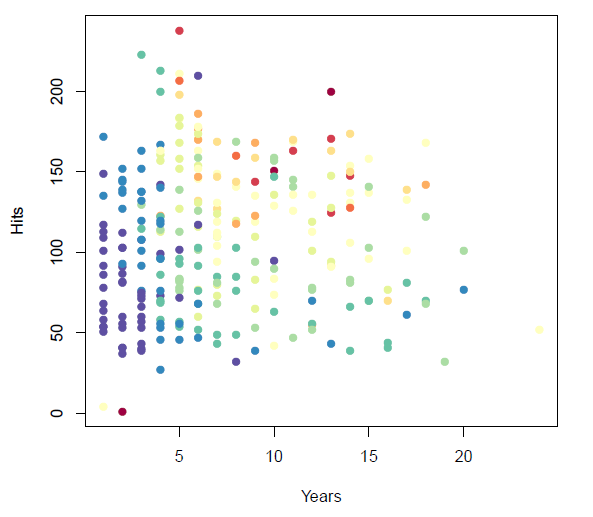
\includegraphics[width=0.60000\textwidth]{hits.png}

\end{block}

\end{frame}

\begin{frame}

\begin{block}{Main idea of tree-based methods}

\begin{itemize}
\item
  We can divide the area into rectangles with similar salaries.
\item
  Do this by deriving a set of decision (splitting) rules for segmenting
  the predictor space into a number of finer and finer regions.
\item
  All points in the same region will be given the same predictive value
  (the mean of all values in that square, or a majority vote).
\end{itemize}

In two dimensions (for two variables) a three-region partition may look
like this:

\centering
\includegraphics[width=0.50000\textwidth]{../../ISLR/Figures/Chapter8/8.2.png}

\end{block}

\end{frame}

\begin{frame}

The series of splitting rules can be visualized with a \emph{regression
tree}.

The following tree (which corresponds to the split in the previous
slide) has three \emph{leaves} (terminal nodes), and two \emph{internal
nodes}:

\(~\)

\centering

\includegraphics[width=0.50000\textwidth]{../../ISLR/Figures/Chapter8/8.1.png}

\end{frame}

\begin{frame}

\begin{block}{More than two predictors?}

\vspace{2mm}

\begin{itemize}
\item
  With more than two predictors we cannot draw the partition of the data
  in a coordinate system, but we can still draw the regression tree.
\item
  Before we discuss how the algorithm splits the data into regions, let
  us look at a somewhat more interesting example.
\end{itemize}

\end{block}

\end{frame}

\begin{frame}

\begin{block}{Example 2: Detection of Minor Head Injury}

\tiny
(Artificial data) \vspace{2mm}

\normalsize

\begin{itemize}
\item
  Data from patients that enter hospital. The aim is to quickly assess
  whether a patient as a brain injury or not.
\item
  Patients are investigated and (possible) asked questions.
\item
  Our job: To build a good model to predict quickly if someone has a
  brain injury. The method should be

  \begin{itemize}
  \item
    \textbf{easy} to interpret for the medical personell that are not
    skilled in statistics, and
  \item
    \textbf{fast}, such that the medical personell quickly can identify
    a patient that needs treatment.
  \end{itemize}
\end{itemize}

\(\rightarrow\) This can be done by using tree-based methods.

\vspace{4mm}

\small
Note: Of course, the model should be built \emph{before} a new emergency
patient arrives, using data that is already available.

\end{block}

\end{frame}

\begin{frame}[fragile]

The dataset includes data about 1321 patients and is a modified and
smaller version of the (simulated) dataset \texttt{headInjury} from the
\texttt{DAAG} library.

\footnotesize

\begin{verbatim}
##    amnesia bskullf GCSdecr GCS.13 GCS.15 risk consc oskullf vomit
## 3        0       0       0      0      0    0     0       0     0
## 9        0       0       0      0      0    1     0       0     0
## 11       0       0       0      0      0    0     0       0     0
## 12       1       0       0      0      0    0     0       0     0
## 14       0       0       0      0      0    0     0       0     0
## 16       0       0       0      0      0    0     0       0     0
##    brain.injury age
## 3             0  44
## 9             0  67
## 11            0  62
## 12            0   1
## 14            0  55
## 16            0  63
\end{verbatim}

\normalsize

\end{frame}

\begin{frame}[fragile]

\begin{itemize}
\tightlist
\item
  The variable \texttt{brain.injury} will be the response of our model:
  It has value 1 if a person has an acute brain injury, and 0 otherwise.
\end{itemize}

\vspace{0mm}

\begin{itemize}
\tightlist
\item
  250 (19\%) of the patients have a clinically important brain injury.
\end{itemize}

\vspace{0mm}

\begin{itemize}
\item
  The 10 variables used as explanatory variables describe the state of
  the patient, for example

  \begin{itemize}
  \tightlist
  \item
    Is he/she vomiting?
  \item
    Is the Glasgow Coma Scale (GCS)
    score\footnote{The GCS scale goes back to an article in the Lancet in 1974, and is used to describe the level of consciousness of patients with an acute brain injury. See <https://www.glasgowcomascale.org/what-is-gcs/>}
    after 2 hours equal to 15 (or not)?
  \item
    Has he/she an open scull fracture?
  \item
    Has he/she had a loss of consciousness?
  \item
    and so on.
  \end{itemize}
\end{itemize}

\end{frame}

\begin{frame}

The classification tree made from a training set of 850 randomly drawn
observations (training set) for the head injury example looks like this:

\begin{center}\includegraphics[width=0.7\linewidth]{8Trees_files/figure-beamer/injury1-1} \end{center}

\small
Note: The split criterion at each node is to the left. For example,
``GCS.15:0'' means that ``GCS.15=0'' goes left, and ``GCS.15=1'' goes
right.

\end{frame}

\begin{frame}[fragile]

\footnotesize

\begin{Shaded}
\begin{Highlighting}[]
\KeywordTok{print}\NormalTok{(headtree)}
\end{Highlighting}
\end{Shaded}

\begin{verbatim}
## node), split, n, deviance, yval, (yprob)
##       * denotes terminal node
## 
##  1) root 850 819.00 0 ( 0.8129 0.1871 )  
##    2) GCS.15: 0 711 520.00 0 ( 0.8805 0.1195 )  
##      4) bskullf: 0 663 398.00 0 ( 0.9110 0.0890 )  
##        8) risk: 0 487 203.00 0 ( 0.9466 0.0534 )  
##         16) age < 68.5 445 131.00 0 ( 0.9663 0.0337 ) *
##         17) age > 68.5 42  48.30 0 ( 0.7381 0.2619 ) *
##        9) risk: 1 176 170.00 0 ( 0.8125 0.1875 ) *
##      5) bskullf: 1 48  66.20 1 ( 0.4583 0.5417 )  
##       10) age < 42.5 13  11.20 0 ( 0.8462 0.1538 ) *
##       11) age > 42.5 35  43.60 1 ( 0.3143 0.6857 ) *
##    3) GCS.15: 1 139 192.00 1 ( 0.4676 0.5324 )  
##      6) GCS.13: 0 121 167.00 0 ( 0.5289 0.4711 )  
##       12) risk: 0 78 101.00 0 ( 0.6538 0.3462 )  
##         24) age < 66.5 66  77.30 0 ( 0.7273 0.2727 ) *
##         25) age > 66.5 12  13.50 1 ( 0.2500 0.7500 ) *
##       13) risk: 1 43  52.70 1 ( 0.3023 0.6977 ) *
##      7) GCS.13: 1 18   7.72 1 ( 0.0556 0.9444 ) *
\end{verbatim}

\normalsize

\end{frame}

\begin{frame}

\begin{itemize}
\item
  By using simple decision rules related to the most important
  explanatory variables the medical staff can now assess the probability
  of a brain injury.
\item
  The decision can go ``top down'', because the most informative
  predictors are usually split first.
\item
  Example: The staff might check if the Glasgow Coma Scale of the
  patient is 15 after 2h, and if it was 13 at the beginning. In that
  case, the probability of brain injury is estimated to be 0.944 (node 7
  in printout).
\end{itemize}

\textbf{Advantages}:

\begin{itemize}
\item
  Decisions trees are easier to interpret than many of the
  classification (and regression) methods that we have studied so far.
\item
  Decisions trees provide an easy way to visualize the data for
  non-statisticians.
\end{itemize}

\end{frame}

\begin{frame}

\begin{block}{Glossary}

\begin{itemize}
\item
  Classification and regression trees are usually drawn upside down,
  where the top node is called the \emph{root}.
\item
  The \emph{terminal nodes} or \emph{leaf nodes} are the nodes at the
  bottom, with no splitting criteria. These represent the final
  predicted class (for classification trees) or predicted response value
  (for regression trees) and are written symbolically as \(R_j\) for
  \(j = 1, 2, ..., J\)
\item
  The \(R_j\) will be referred to as \emph{non-overlapping regions}.
\item
  \emph{Internal nodes} are all nodes between the root and the terminal
  nodes. These nodes correspond to the partitions of the predictor
  space.
\item
  \emph{Branches}: segment of the tree connecting the nodes.
\end{itemize}

We will consider only binary splits on one variable, but multiway splits
and linear combination of variabes are possible - but not so common.

\end{block}

\end{frame}

\begin{frame}{Constructing a decision tree}

You can construct decision trees for both classification and regression
problems, first we focus on constructing a regression tree.

\begin{block}{Regression tree (continous outcome)}

Assume that we have a dataset consisting of \(n\) pairs
\((\boldsymbol{x}_i,y_i)\), \(i=1,\ldots,n\), and each predictor is
\({\boldsymbol{x}}_i=(x_{i1},x_{i2},...,x_{ip})\). The aim is to predict
\(y_i\).

\vspace{2mm} Two steps:

\begin{enumerate}
\def\labelenumi{\arabic{enumi}.}
\item
  Divide the predictor space into non-overlapping regions
  \(R_1,R_2,\ldots,R_J\).
\item
  For every observation that falls into region \(R_j\) we make the same
  prediction - which is the mean of the responses for the training
  observations that fall into \(R_j\).
\end{enumerate}

\vspace{2mm}

\textbf{But}: How to divide the predictor space into non-overlapping
regions \(R_1,R_2,\ldots,R_J\)?

\end{block}

\end{frame}

\begin{frame}

We could try to minimize the RSS (residual sums of squares) on the
training set given by

\[
\text{RSS}=\sum_{j=1}^J \sum_{i \in R_j}(y_i-\hat{y}_{R_j})^2,
\]

where \(\hat{y}_{R_j}\) is the mean response for the training
observations in region \(j\). The mean \(\hat{y}_{R_j}\) is also the
predicted value for a new observations that falls into region \(j\).

To do this we need to consider every partition of the predictor space,
and compute the RSS for each partition.

\textbf{But}: An exhaustive search over possible splits is
\emph{computationally infeasible}! In fact, constructing optimal binary
decision tress is an NP-complete problem (Hyafil and Rivest 1976).

\end{frame}

\begin{frame}

\begin{block}{Recursive binary splitting}

\vspace{2mm}

\begin{itemize}
\item
  A \emph{greedy} approach is taken (aka top-down) - called
  \emph{recursive binary splitting.} The idea is to find a split that
  minimizes RSS at each step.
\item
  We start at the top of the tree and divide the predictor space into
  two regions, \(R_1\) and \(R_2\) by making a decision rule for one of
  the predictors \(x_1, x_2,...,x_p\). If we define the two regions by
  \(R_1(j,s)=\{x \mid x_j<s\}\) and \(R_2(j,s)=\{x \mid x_j\geq s\}\),
  it means that we need to find the (predictor) \(j\) and (splitting
  point) \(s\) that minimize
  \[\sum_{i: x_i \in R_1(j,s)}(y_i-\hat{y}_{R_1})^2+\sum_{i: x_i \in R_2(j,s)}(y_i -\hat{y}_{R_2})^2 \ ,\]
  where \(\hat{y}_{R_1}\) and \(\hat{y}_{R_2}\) are the mean responses
  for the training observations in \(R_1(j,s)\) and \(R_2(j,s)\)
  respectively. This way we get the two first branches in our decision
  tree.
\end{itemize}

\end{block}

\end{frame}

\begin{frame}

\begin{itemize}
\item
  We repeat the process to make branches further down in the tree.
\item
  For every iteration we let each single split depend on \emph{only one
  of the predictors}, giving us two new branches.
\item
  This is done \emph{successively} and in each step we choose the split
  that gives the
  \emph{\textcolor{red}{best split at that particular step}},
  \emph{i.e.,} the split that gives the smallest RSS.
\item
  Continue splitting the predictor space until we reach some
  \emph{stopping criterion}. For example we stop when a region contains
  less than 10 observations or when the reduction in the RSS is smaller
  than a specified limit.
\end{itemize}

\vspace{1mm}

\textbf{Q}: Why is this algorithm called \emph{greedy}?

\end{frame}

\begin{frame}[fragile]

\begin{block}{Regression tree: ozone example}

\vspace{2mm}

Consider the \texttt{ozone} data set from the \texttt{ElemStatLearn}
library. The data set consists of 111 observations on the following
variables:

\begin{itemize}
\tightlist
\item
  \texttt{ozone} : the concentration of ozone in ppb
\item
  \texttt{radiation}: the solar radiation (langleys)
\item
  \texttt{temperature} : the daily maximum temperature in degrees F
\item
  \texttt{wind} : wind speed in mph
\end{itemize}

\begin{Shaded}
\begin{Highlighting}[]
\KeywordTok{head}\NormalTok{(myozone)}
\end{Highlighting}
\end{Shaded}

\begin{verbatim}
##   ozone radi temp wind
## 1    41  190   67  7.4
## 2    36  118   72  8.0
## 3    12  149   74 12.6
## 4    18  313   62 11.5
## 5    23  299   65  8.6
## 6    19   99   59 13.8
\end{verbatim}

\end{block}

\end{frame}

\begin{frame}[fragile]

Suppose we want to get an estimate of the ozone concentration based on
the measurement of wind speed and the daily maximum temperature.

\(\rightarrow\) We can fit a regression tree to the data, with
\texttt{ozone} as our response variable and \texttt{temperature} and
\texttt{wind} as predictors (not including radiation to make this easier
to see). This gives us the following regression tree.

\end{frame}

\begin{frame}[fragile]

\footnotesize

\begin{Shaded}
\begin{Highlighting}[]
\NormalTok{ozone.trainID =}\StringTok{ }\KeywordTok{sample}\NormalTok{(}\DecValTok{1}\OperatorTok{:}\DecValTok{111}\NormalTok{, }\DecValTok{75}\NormalTok{)}
\NormalTok{ozone.train =}\StringTok{ }\NormalTok{myozone[ozone.trainID, ]}
\NormalTok{ozone.test =}\StringTok{ }\NormalTok{myozone[}\OperatorTok{-}\NormalTok{ozone.trainID, ]}
\CommentTok{# use the default settings in the tree function:}
\NormalTok{ozone.tree =}\StringTok{ }\KeywordTok{tree}\NormalTok{(ozone }\OperatorTok{~}\StringTok{ }\NormalTok{temp }\OperatorTok{+}\StringTok{ }\NormalTok{wind, }\DataTypeTok{data =}\NormalTok{ ozone.train)}
\end{Highlighting}
\end{Shaded}

\begin{center}\includegraphics[width=0.6\linewidth]{8Trees_files/figure-beamer/ozone1-1} \end{center}

\end{frame}

\begin{frame}[fragile]

\begin{itemize}
\item
  We see that \texttt{temperature} is the ``most important'' predictor
  for predicting the ozone concentration. Observe that we can split on
  the same variable several times.
\item
  Focus on the regions \(R_j\), \(j=1,\ldots, J\). What is \(J\) here?
  Answer: \(J=6\) (= the number of leaf nodes).
\end{itemize}

\vspace{2mm} Below we see the partition of the \texttt{ozone} data set
given in the \texttt{ozone.tree}, where

\begin{itemize}
\tightlist
\item
  the ozone levels have been color-coded, where a darker color
  corresponds to a higher ozone concentration.
\item
  each rectangle corresponds to one leaf node.
\item
  each number corresponding to a leaf node has been found by taking an
  average of all observations (in the training set) in the corresponding
  region (rectangle).
\item
  each partition line corresponds to one internal node of a binary
  partition.
\end{itemize}

\end{frame}

\begin{frame}

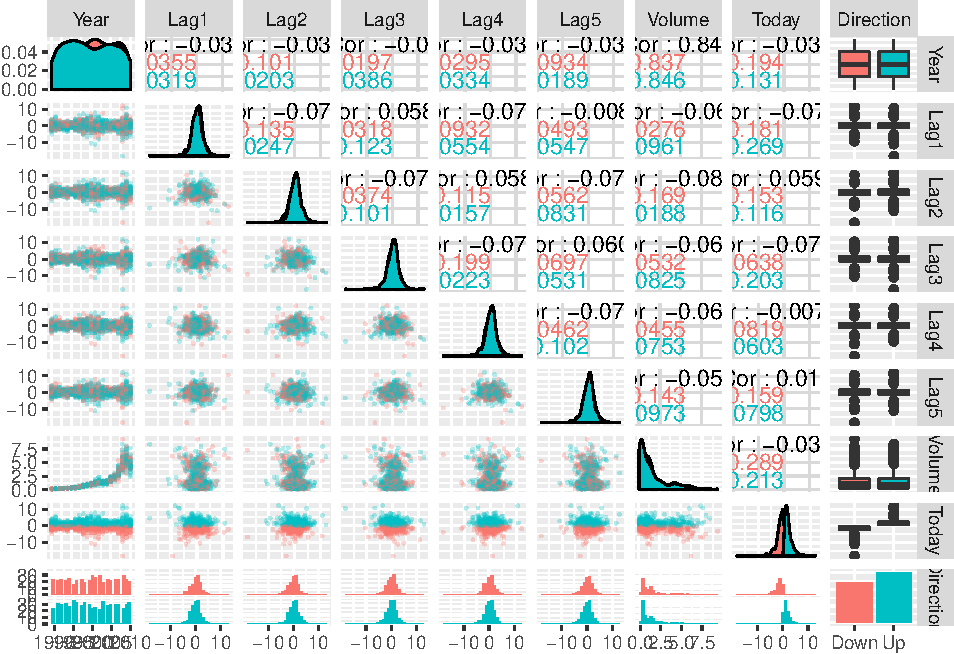
\includegraphics{8Trees_files/figure-beamer/unnamed-chunk-6-1.pdf}

\textbf{Q}:

\begin{itemize}
\tightlist
\item
  Explain the connection between the tree and the region plot.
\item
  Why is recursive binary splitting classified as a greedy algorithm?
\item
  Discuss the advantages and disadvantages of letting each single split
  depend on only one of the predictors.
\item
  Does our tree automatically include interactions between variables?
\end{itemize}

\end{frame}

\begin{frame}

\textbf{A:}

\begin{itemize}
\tightlist
\item
  Each leaf node correspons to one region with prediction
  \(\hat{y}_{R_j}\), and each internal note corresponds to a vertical or
  a horizontal line.
\item
  Recursive splitting does not necessarily give the optimal global
  solution, but will give the best solution at each split (given what is
  done previously).
\item
  If the true connection between the response onzone and temperature and
  wind was so that splits should have been made on the diagonal of the
  temperature and wind space, that would take many splits on each of
  temperature and wind to produce. (See more below where we ask the same
  question for the classification setting.)
\item
  Yes, we may have different effect of wind for different values of
  temperature.
\end{itemize}

\end{frame}

\begin{frame}[fragile]

\begin{block}{R: function \texttt{tree} in library \texttt{tree}}

\vspace{2mm}

\begin{itemize}
\item
  R package \texttt{tree} by Brian D. Ripley (B. Ripley 2019).
\item
  You get information about the function when you type \texttt{?tree}
  into the \texttt{R} console.
\item
  Note: The default choice for a function to minimize is the deviance,
  and for normal data (as we may assume for regression), the deviance is
  proportional to the RSS.
\end{itemize}

\begin{itemize}
\tightlist
\item
  A competing R function is \texttt{rpart}, explained in
  \url{https://cran.r-project.org/web/packages/rpart/vignettes/longintro.pdf}
\end{itemize}

\end{block}

\end{frame}

\begin{frame}[fragile]

\begin{block}{Stopping criterion}

\vspace{2mm}

\begin{itemize}
\item
  When building the tree, we can (in principle) split until each leaf
  corresponds to one data point.
\item
  Usually we use a less stringent stopping criterion, like the minimal
  number of nodes per region and/or the minimum reduction in the RSS.
\item
  For example, the default in \texttt{tree()}: is given by
  \texttt{mincut=5,\ minsize=10,\ mindev=0.01}, thus a minimal size of 5
  nodes and the minimal reduction in deviance (RSS) equal to 0.01.
\item
  We could make the ozone tree much deeper by decreasing the minimal
  size of a region and chanding the minimum reduction in RSS:
\end{itemize}

\scriptsize

\begin{Shaded}
\begin{Highlighting}[]
\NormalTok{ozone.tree2 =}\StringTok{ }\KeywordTok{tree}\NormalTok{(ozone }\OperatorTok{~}\StringTok{ }\NormalTok{temp }\OperatorTok{+}\StringTok{ }\NormalTok{wind, }\DataTypeTok{data =}\NormalTok{ ozone.train, }\DataTypeTok{control =} \KeywordTok{tree.control}\NormalTok{(}\DecValTok{75}\NormalTok{, }
    \DataTypeTok{mincut =} \DecValTok{2}\NormalTok{, }\DataTypeTok{minsize =} \DecValTok{4}\NormalTok{, }\DataTypeTok{mindev =} \FloatTok{0.001}\NormalTok{))}
\end{Highlighting}
\end{Shaded}

\end{block}

\end{frame}

\begin{frame}

With the above command, the tree would become very fine. Overfitting?

\begin{center}\includegraphics[width=0.7\linewidth]{8Trees_files/figure-beamer/ozone2-1} \end{center}

\end{frame}

\begin{frame}[fragile]

\begin{block}{Tree performance}

\vspace{2mm}

To test the predictive performance of our regression tree, we have
randomly divided our observations into a test and a training set (here
1/3 test). For the two trees (the shallow and the deep one from above),
we get the following test MSEs:

\begin{Shaded}
\begin{Highlighting}[]
\NormalTok{ozone.pred =}\StringTok{ }\KeywordTok{predict}\NormalTok{(ozone.tree, }\DataTypeTok{newdata =}\NormalTok{ ozone.test)}
\NormalTok{ozone.MSE =}\StringTok{ }\KeywordTok{mean}\NormalTok{((ozone.pred }\OperatorTok{-}\StringTok{ }\NormalTok{ozone.test}\OperatorTok{$}\NormalTok{ozone)}\OperatorTok{^}\DecValTok{2}\NormalTok{)}
\NormalTok{ozone.MSE}
\end{Highlighting}
\end{Shaded}

\begin{verbatim}
## [1] 384.491
\end{verbatim}

\begin{Shaded}
\begin{Highlighting}[]
\NormalTok{ozone.pred2 =}\StringTok{ }\KeywordTok{predict}\NormalTok{(ozone.tree2, }\DataTypeTok{newdata =}\NormalTok{ ozone.test)}
\NormalTok{ozone.MSE2 =}\StringTok{ }\KeywordTok{mean}\NormalTok{((ozone.pred2 }\OperatorTok{-}\StringTok{ }\NormalTok{ozone.test}\OperatorTok{$}\NormalTok{ozone)}\OperatorTok{^}\DecValTok{2}\NormalTok{)}
\NormalTok{ozone.MSE2}
\end{Highlighting}
\end{Shaded}

\begin{verbatim}
## [1] 491.266
\end{verbatim}

\vspace{1mm}

\textbf{How do we know if our tree performs good, or if there would be
trees with a better predictive performance?}

\end{block}

\end{frame}

\begin{frame}{Pruning}

\begin{itemize}
\item
  If we have a data set with many predictors or choose a stringent
  stopping criterion, we may fit a (too) large tree. Thus, the number of
  observations from the training set that falls into some of the regions
  \(R_j\) may be small \(\rightarrow\)
  \emph{\textcolor{red}{overfitting}}?
\item
  A smaller tree with fewer splits leads to fewer regions
  \(R_1, \ldots, R_J\) with more observations. This might lead to lower
  variance and better interpretation at the cost of a little bias.
\item
  One possible alternative to the process described above is to grow the
  tree only so long as the decrease in the RSS due to each split exceeds
  some (high) threshold.
\item
  This strategy will result in smaller trees, but is too short-sighted:
  a seemingly worthless split early on in the tree might be followed by
  a very good split --- that is, a split that leads to a large reduction
  in RSS later on.
\end{itemize}

\end{frame}

\begin{frame}

\begin{block}{Cost complexity pruning}

\begin{itemize}
\item
  Better idea: to grow a very large tree \(T_0\), and then
  \emph{\textcolor{red}{prune}} it back in order to obtain a subtree
\item
  \emph{\textcolor{red}{Cost complexity pruning}} is used for this: We
  try to find a subtree \(T\subset T_0\) that (for a given value of
  \(\alpha\)) minimizes \[
  C_{\alpha}(T)=Q(T)+\alpha |T|,
  \] where \(Q(T)\) is our cost function, \(|T|\) is the number of
  terminal nodes in tree \(T\). The parameter \(\alpha\) is then a
  parameter penalizing the number of terminal nodes, ensuring that the
  tree does not get too many branches.
\item
  For regression trees we choose
  \[Q(T)=\sum_{m=1}^{|T|}\sum_{x_i\in R_m}(y_i - \hat{y}_{R_m})^2 \ ,\]
  and adapted cost functions for classification trees (the entropy
  (deviance), Gini or misclassification rate, see below).
\end{itemize}

\end{block}

\end{frame}

\begin{frame}

\begin{itemize}
\item
  Given a value of \(\alpha\) we get a pruned tree (note: the same
  pruned tree within a small range of \(\alpha\)).
\item
  For \(\alpha=0\) we get \(T_0\) and as \(\alpha\) increases we get
  smaller and smaller trees.
\end{itemize}

So, which value of \(\alpha\) is best?

\begin{itemize}
\item
  We can use \(k\)-fold cross-validation to find out!
\item
  Importantly, by increasing \(\alpha\), branches get pruned in a
  \emph{hierarchical (nested) fashion}.
\end{itemize}

Please study this
\href{https://www.math.ntnu.no/emner/TMA4268/2018v/notes/CART1MA87012017BoLindqvist.pdf}{note
from Bo Lindqvist in MA8701 in 2017 - Advanced topics in Statistical
Learning and Inference} for an example of how we perform cost complexity
pruning in detail. Alterntively, this method, with proofs, are given in
B. D. Ripley (1996), Section 7.2.

\end{frame}

\begin{frame}

\begin{block}{Pruning the ozone tree}

Let us start with the tree with many leafes, and then prune it with
5-fold CV. We can then plot the CV error as a function of tree size
(instead of \(\alpha\) -- why?):

\begin{center}\includegraphics[width=0.6\linewidth]{8Trees_files/figure-beamer/ozone.cv-1} \end{center}

Interestingly, it seems like a tree with 5 leafes performs best - which
corresponds to the original choice.

\end{block}

\end{frame}

\begin{frame}{Classification trees (binary or categorical outcome)}

\vspace{2mm}

\begin{itemize}
\tightlist
\item
  Remember the minor head injury example: Binary outcome (disease
  yes/no).
\end{itemize}

\vspace{1mm}

\begin{itemize}
\tightlist
\item
  Now allow for \(K\geq 2\) number of classes for the response.
\end{itemize}

\vspace{1mm}

\begin{itemize}
\tightlist
\item
  Building a decision tree in this setting is similar to building a
  regression tree for a quantitative response, but there are two main
  differences: \emph{the prediction} and \emph{the splitting criterion}.
\end{itemize}

\end{frame}

\begin{frame}

\textbf{1) The prediction:}

\begin{itemize}
\item
  In the regression case we use the mean value of the responses in
  \(R_j\) as a prediction for an observation that falls into region
  \(R_j\).
\item
  For the \emph{\textcolor{red}{classification case}}, however, we have
  two possibilities:

  \begin{itemize}
  \tightlist
  \item
    Majority vote: Predict that the observation belongs to the most
    commonly occurring class of the training observations in \(R_j\).\\
  \item
    Estimate the probability that an observation \(x_i\) belongs to a
    class \(k\), \(\hat{p}_{jk}(x_i)\), and then classify according to a
    threshold value. This estimated probability is the proportion of
    class \(k\) training observations in region \(R_j\), with \(n_{jk}\)
    observations. Region \(j\) has \(N_j\) observations.
    \[\hat{p}_{jk} = \frac{1}{N_j} \sum_{i:x_i \in R_j} I(y_i = k)=\frac{n_{jk}}{N_j}.\]
  \end{itemize}
\end{itemize}

\end{frame}

\begin{frame}

\textbf{2) The splitting criterion:} We do not use RSS as a splitting
criterion for a qualitative variable. Instead we can use some
\emph{measure of impurity} of the node. For leaf node \(j\) and class
\(k=1,\ldots, K\):

\begin{itemize}
\tightlist
\item
  \textbf{Gini index}: \[
  G=\sum_{k=1}^K \hat{p}_{jk}(1-\hat{p}_{jk}) \ ,
  \] which is small if all of the \(\hat{p}_{jk}\)'s are close to 0 or
  1.
\end{itemize}

\vspace{1mm}

\begin{itemize}
\tightlist
\item
  \textbf{Cross entropy}: \[
  D=-\sum_{k=1}^K \hat{p}_{jk}\log\hat{p}_{jk} \ .
  \] Here \(\hat{p}_{jk}\) is the proportion of training observation in
  region \(j\) that are from class \(k\).
\end{itemize}

When making a split in our classification tree, we want to minimize the
Gini index or the cross-entropy.

\end{frame}

\begin{frame}

Why don't we just minimize the misclassification error
\[E= 1- \max_k{\hat{p}_{jk}} \ ?\]

\textbf{A}: The Gini index and Entropy are \emph{measure of impurity}.
Moreover, they are differentiable (preferred for numerical
optimization!).

\begin{center}\includegraphics[width=0.7\linewidth]{8Trees_files/figure-beamer/purity-1} \end{center}

\end{frame}

\begin{frame}[fragile]

\begin{block}{Minor head injury - split with cross-entropy}

\footnotesize

\begin{Shaded}
\begin{Highlighting}[]
\NormalTok{tree.HIClass =}\StringTok{ }\KeywordTok{tree}\NormalTok{(brain.injury }\OperatorTok{~}\StringTok{ }\NormalTok{., }\DataTypeTok{data =}\NormalTok{ headInjury2, }\DataTypeTok{subset =}\NormalTok{ train, }
    \DataTypeTok{split =} \StringTok{"deviance"}\NormalTok{)}
\KeywordTok{summary}\NormalTok{(tree.HIClass)}
\end{Highlighting}
\end{Shaded}

\begin{verbatim}
## 
## Classification tree:
## tree(formula = brain.injury ~ ., data = headInjury2, subset = train, 
##     split = "deviance")
## Variables actually used in tree construction:
## [1] "GCS.15"  "bskullf" "risk"    "age"     "GCS.13" 
## Number of terminal nodes:  9 
## Residual mean deviance:  0.6604 = 555.4 / 841 
## Misclassification error rate: 0.1259 = 107 / 850
\end{verbatim}

\normalsize

Remark: the deviance is a scaled version of the cross entropy:
\(-2\sum_{k=1}^K n_{jk} \log\hat{p}_{jk}\) where
\(\hat{p}_{jk}=\frac{n_{jk}}{N_j}\), thus \texttt{split="deviance"}
implies that we split according to the entropy criterion.

\end{block}

\end{frame}

\begin{frame}[fragile]

\begin{Shaded}
\begin{Highlighting}[]
\KeywordTok{plot}\NormalTok{(tree.HIClass, }\DataTypeTok{type =} \StringTok{"proportional"}\NormalTok{)}
\KeywordTok{text}\NormalTok{(tree.HIClass, }\DataTypeTok{pretty =} \DecValTok{1}\NormalTok{)}
\end{Highlighting}
\end{Shaded}

\begin{center}\includegraphics[width=0.7\linewidth]{8Trees_files/figure-beamer/headInjury-1} \end{center}

Note: With \texttt{type="proportional"}, the length of branches are now
proportional to the decrease in impurity.

\end{frame}

\begin{frame}[fragile]

\begin{block}{Minor head injury - split with Gini index}

\footnotesize

\begin{Shaded}
\begin{Highlighting}[]
\NormalTok{tree.HIClassG =}\StringTok{ }\KeywordTok{tree}\NormalTok{(brain.injury }\OperatorTok{~}\StringTok{ }\NormalTok{., headInjury2, }\DataTypeTok{subset =}\NormalTok{ train, }
    \DataTypeTok{split =} \StringTok{"gini"}\NormalTok{)}
\KeywordTok{summary}\NormalTok{(tree.HIClassG)}
\end{Highlighting}
\end{Shaded}

\begin{verbatim}
## 
## Classification tree:
## tree(formula = brain.injury ~ ., data = headInjury2, subset = train, 
##     split = "gini")
## Variables actually used in tree construction:
## [1] "GCS.15"  "bskullf" "risk"    "age"     "oskullf" "vomit"   "amnesia"
## [8] "consc"   "GCS.13" 
## Number of terminal nodes:  75 
## Residual mean deviance:  0.5202 = 403.2 / 775 
## Misclassification error rate: 0.1094 = 93 / 850
\end{verbatim}

\normalsize

\end{block}

\end{frame}

\begin{frame}[fragile]

\footnotesize

\begin{Shaded}
\begin{Highlighting}[]
\NormalTok{tree.HIClassG =}\StringTok{ }\KeywordTok{tree}\NormalTok{(brain.injury }\OperatorTok{~}\StringTok{ }\NormalTok{., headInjury2, }\DataTypeTok{subset =}\NormalTok{ train, }
    \DataTypeTok{split =} \StringTok{"gini"}\NormalTok{)}
\KeywordTok{plot}\NormalTok{(tree.HIClassG)}
\KeywordTok{text}\NormalTok{(tree.HIClassG, }\DataTypeTok{pretty =} \DecValTok{1}\NormalTok{)}
\end{Highlighting}
\end{Shaded}

\begin{center}\includegraphics[width=0.85\linewidth]{8Trees_files/figure-beamer/headInjury2-1} \end{center}

\end{frame}

\begin{frame}[fragile]

We also use the classification tree to predict the status of the
patients in the test set (the one grown with deviance)

\tiny

\begin{Shaded}
\begin{Highlighting}[]
\KeywordTok{library}\NormalTok{(caret)}
\NormalTok{tree.pred =}\StringTok{ }\KeywordTok{predict}\NormalTok{(tree.HIClass, headInjury2[test, ], }\DataTypeTok{type =} \StringTok{"class"}\NormalTok{)}
\KeywordTok{confusionMatrix}\NormalTok{(tree.pred, }\DataTypeTok{reference =}\NormalTok{ headInjury2[test, ]}\OperatorTok{$}\NormalTok{brain.injury)}
\end{Highlighting}
\end{Shaded}

\begin{verbatim}
## Confusion Matrix and Statistics
## 
##           Reference
## Prediction   0   1
##          0 356  42
##          1  24  49
##                                           
##                Accuracy : 0.8599          
##                  95% CI : (0.8252, 0.8899)
##     No Information Rate : 0.8068          
##     P-Value [Acc > NIR] : 0.001545        
##                                           
##                   Kappa : 0.514           
##                                           
##  Mcnemar's Test P-Value : 0.036389        
##                                           
##             Sensitivity : 0.9368          
##             Specificity : 0.5385          
##          Pos Pred Value : 0.8945          
##          Neg Pred Value : 0.6712          
##              Prevalence : 0.8068          
##          Detection Rate : 0.7558          
##    Detection Prevalence : 0.8450          
##       Balanced Accuracy : 0.7377          
##                                           
##        'Positive' Class : 0               
## 
\end{verbatim}

\end{frame}

\begin{frame}[fragile]

And for the Gini-grown tree

\tiny

\begin{Shaded}
\begin{Highlighting}[]
\NormalTok{tree.predG =}\StringTok{ }\KeywordTok{predict}\NormalTok{(tree.HIClassG, headInjury2[test, ], }\DataTypeTok{type =} \StringTok{"class"}\NormalTok{)}
\KeywordTok{confusionMatrix}\NormalTok{(tree.predG, }\DataTypeTok{reference =}\NormalTok{ headInjury2[test, ]}\OperatorTok{$}\NormalTok{brain.injury)}
\end{Highlighting}
\end{Shaded}

\begin{verbatim}
## Confusion Matrix and Statistics
## 
##           Reference
## Prediction   0   1
##          0 354  47
##          1  26  44
##                                           
##                Accuracy : 0.845           
##                  95% CI : (0.8091, 0.8765)
##     No Information Rate : 0.8068          
##     P-Value [Acc > NIR] : 0.01855         
##                                           
##                   Kappa : 0.455           
##                                           
##  Mcnemar's Test P-Value : 0.01924         
##                                           
##             Sensitivity : 0.9316          
##             Specificity : 0.4835          
##          Pos Pred Value : 0.8828          
##          Neg Pred Value : 0.6286          
##              Prevalence : 0.8068          
##          Detection Rate : 0.7516          
##    Detection Prevalence : 0.8514          
##       Balanced Accuracy : 0.7075          
##                                           
##        'Positive' Class : 0               
## 
\end{verbatim}

\end{frame}

\begin{frame}

\begin{block}{Questions:}

\begin{itemize}
\tightlist
\item
  The classification tree has two terminal nodes with factor ``1''
  originating from the same branch. Why do we get this ``unnecessary''
  split?
\item
  What if we have \(x_1\) and \(x_2\) and the true class boundary (two
  classes) is linear in \(x_1\), \(x_2\) space. How can we do that with
  our binary recursive splits?
\end{itemize}

\end{block}

\end{frame}

\begin{frame}

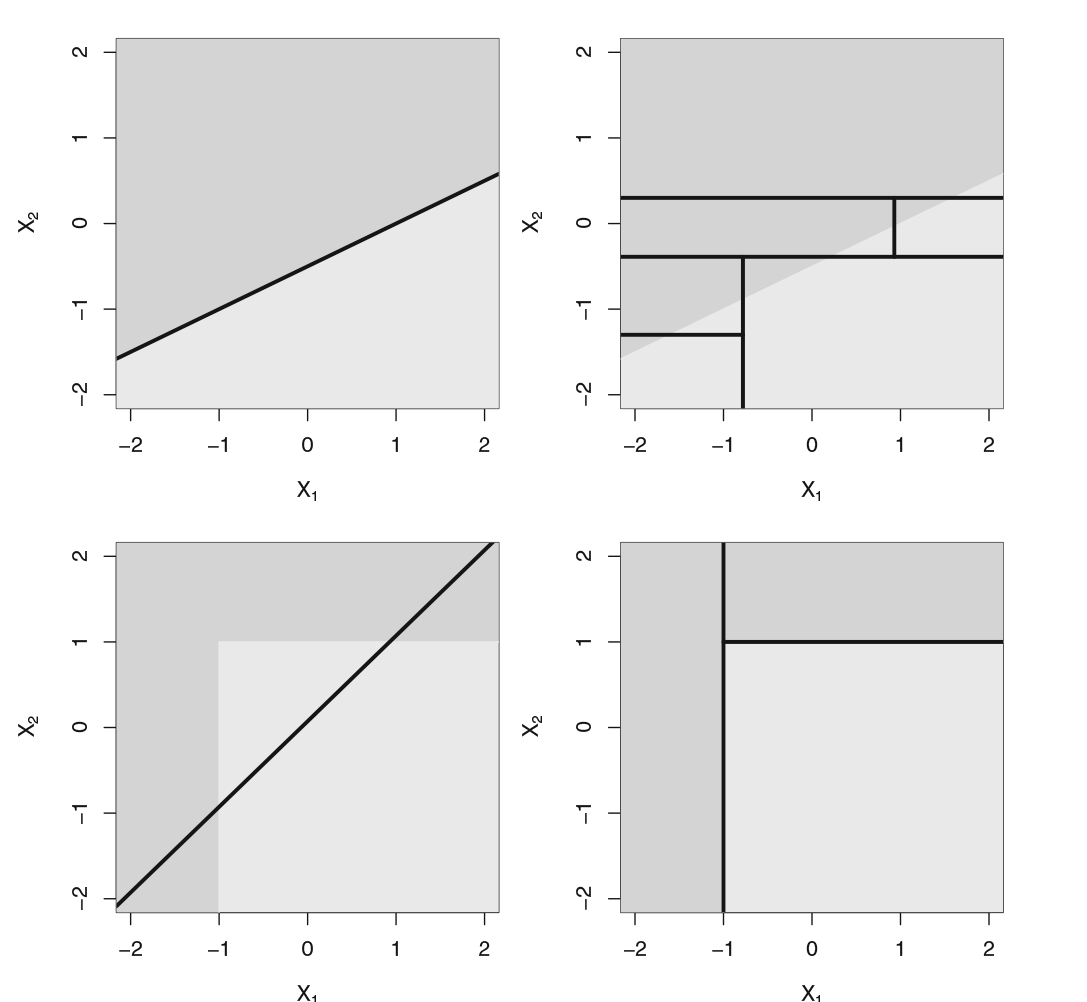
\includegraphics{Introtostatlearn-326.png}

\end{frame}

\begin{frame}

\begin{itemize}
\tightlist
\item
  What about a rectangular boundary (figure above)?
\item
  Study the above confusion matrices. One type of mistake is more severe
  than the other. Discuss if it is possible to change the algorithm in
  order to decrease the number of severe mistakes.
\end{itemize}

\end{frame}

\begin{frame}

\begin{block}{Building a regression (classification) tree: Algorithm
8.1}

\begin{enumerate}
\def\labelenumi{\arabic{enumi}.}
\tightlist
\item
  Use recursive binary splitting to grow a large tree on the training
  data, stopping only when each terminal node has fewer than some
  minimum number of observations.
\item
  Apply cost complexity pruning to the large tree in order to obtain a
  sequence of best subtrees, as a function of \(\alpha\).
\item
  Use K-fold cross-validation to choose \(\alpha\). That is, divide the
  training observations into K folds. For each k = \(1,\ldots, K\):
\end{enumerate}

\begin{itemize}
\tightlist
\item
  Repeat Steps 1 and 2 on all but the kth fold of the training data.
\item
  Evaluate the mean squared prediction (misclassification, gini,
  cross-entropy) error on the data in the left-out kth fold, as a
  function of \(\alpha\).
\item
  Average the results for each value of \(\alpha\), and pick \(\alpha\)
  to minimize the average error.
\end{itemize}

\begin{enumerate}
\def\labelenumi{\arabic{enumi}.}
\setcounter{enumi}{3}
\tightlist
\item
  Return the subtree from Step 2 that corresponds to the chosen value of
  \(\alpha\).
\end{enumerate}

\end{block}

\end{frame}

\begin{frame}[fragile]

\begin{block}{ Combining pruning and cross-validation to find optimal
tree}

We continue using the \href{classtree2}{classification tree}.

\begin{Shaded}
\begin{Highlighting}[]
\KeywordTok{set.seed}\NormalTok{(}\DecValTok{1}\NormalTok{)}
\NormalTok{cv.head =}\StringTok{ }\KeywordTok{cv.tree}\NormalTok{(tree.HIClass, }\DataTypeTok{FUN =}\NormalTok{ prune.misclass)}
\KeywordTok{par}\NormalTok{(}\DataTypeTok{pty =} \StringTok{"s"}\NormalTok{)}
\KeywordTok{plot}\NormalTok{(cv.head}\OperatorTok{$}\NormalTok{size, cv.head}\OperatorTok{$}\NormalTok{dev, }\DataTypeTok{type =} \StringTok{"b"}\NormalTok{, }\DataTypeTok{xlab =} \StringTok{"Terminal nodes"}\NormalTok{, }
    \DataTypeTok{ylab =} \StringTok{"misclassifications"}\NormalTok{)}
\end{Highlighting}
\end{Shaded}

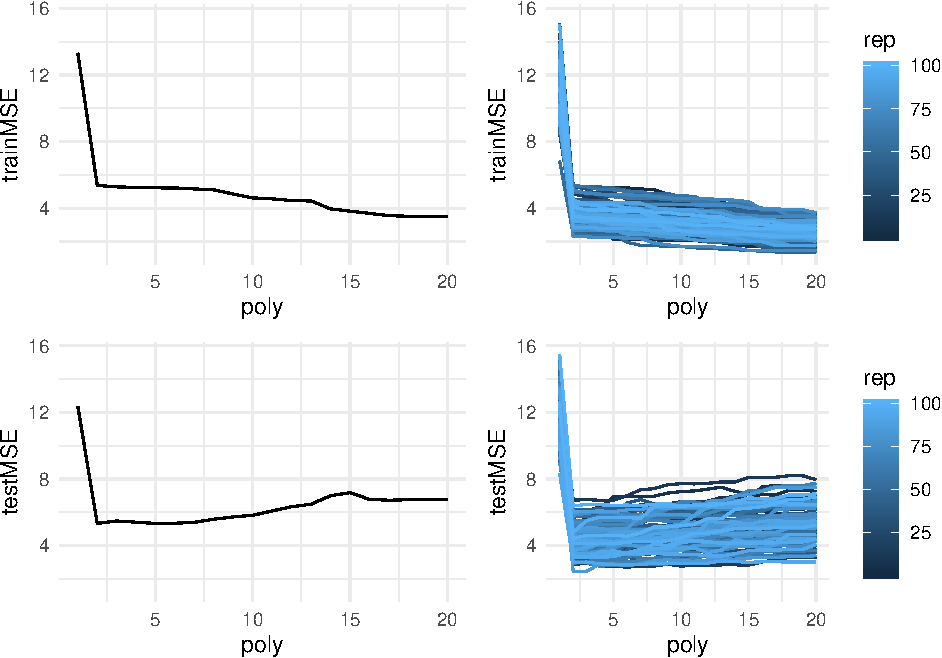
\includegraphics{8Trees_files/figure-beamer/unnamed-chunk-13-1.pdf}

\end{block}

\end{frame}

\begin{frame}[fragile]

The function \texttt{cv.tree} automatically does \(10\)-fold
cross-validation. \texttt{dev} is here the number of misclassifications.

\begin{Shaded}
\begin{Highlighting}[]
\KeywordTok{print}\NormalTok{(cv.head)}
\end{Highlighting}
\end{Shaded}

\begin{verbatim}
## $size
## [1] 9 7 6 4 1
## 
## $dev
## [1] 129 129 149 149 166
## 
## $k
## [1] -Inf  0.0  6.0  6.5 11.0
## 
## $method
## [1] "misclass"
## 
## attr(,"class")
## [1] "prune"         "tree.sequence"
\end{verbatim}

\end{frame}

\begin{frame}[fragile]

We have done cross-validation on our training set of 850 observations.
According to the plot, the number of misclassifications is lowest if we
use 5 terminal nodes. Next, we prune the classification tree according
to this value:

\begin{Shaded}
\begin{Highlighting}[]
\NormalTok{prune.HIClass =}\StringTok{ }\KeywordTok{prune.misclass}\NormalTok{(tree.HIClass, }\DataTypeTok{best =} \DecValTok{5}\NormalTok{)}
\CommentTok{# Five node tree.}
\end{Highlighting}
\end{Shaded}

\end{frame}

\begin{frame}[fragile]

\begin{Shaded}
\begin{Highlighting}[]
\KeywordTok{plot}\NormalTok{(prune.HIClass)}
\KeywordTok{text}\NormalTok{(prune.HIClass, }\DataTypeTok{pretty =} \DecValTok{1}\NormalTok{)}
\end{Highlighting}
\end{Shaded}

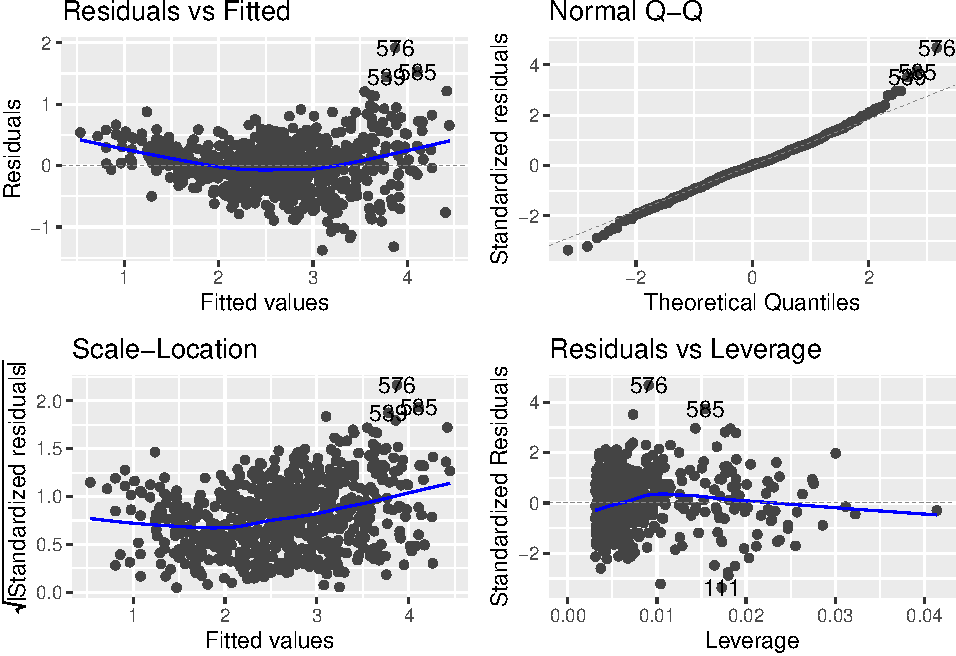
\includegraphics{8Trees_files/figure-beamer/unnamed-chunk-16-1.pdf}

We see that the new tree doesn't have any unnecessary splits, and we
have a simple and interpretable decision tree. How is the predictive
performance of the model affected?

\end{frame}

\begin{frame}[fragile]

\footnotesize

\begin{Shaded}
\begin{Highlighting}[]
\NormalTok{tree.pred.prune =}\StringTok{ }\KeywordTok{predict}\NormalTok{(prune.HIClass, headInjury2[test, ], }\DataTypeTok{type =} \StringTok{"class"}\NormalTok{)}
\KeywordTok{confusionMatrix}\NormalTok{(tree.pred, headInjury2[test, ]}\OperatorTok{$}\NormalTok{brain.injury)}
\end{Highlighting}
\end{Shaded}

\begin{verbatim}
## Confusion Matrix and Statistics
## 
##           Reference
## Prediction   0   1
##          0 356  42
##          1  24  49
##                                           
##                Accuracy : 0.8599          
##                  95% CI : (0.8252, 0.8899)
##     No Information Rate : 0.8068          
##     P-Value [Acc > NIR] : 0.001545        
##                                           
##                   Kappa : 0.514           
##                                           
##  Mcnemar's Test P-Value : 0.036389        
##                                           
##             Sensitivity : 0.9368          
##             Specificity : 0.5385          
##          Pos Pred Value : 0.8945          
##          Neg Pred Value : 0.6712          
##              Prevalence : 0.8068          
##          Detection Rate : 0.7558          
##    Detection Prevalence : 0.8450          
##       Balanced Accuracy : 0.7377          
##                                           
##        'Positive' Class : 0               
## 
\end{verbatim}

\normalsize

We see that the misclassification rate is as small as before indicating
that the pruned tree is as good as the original tree for the test data.

\end{frame}

\begin{frame}[fragile]

The same repeated for the Gini-grown tree - comment on what is done.

\begin{Shaded}
\begin{Highlighting}[]
\KeywordTok{set.seed}\NormalTok{(}\DecValTok{1}\NormalTok{)}
\NormalTok{cv.headG =}\StringTok{ }\KeywordTok{cv.tree}\NormalTok{(tree.HIClassG, }\DataTypeTok{FUN =}\NormalTok{ prune.misclass)}
\KeywordTok{par}\NormalTok{(}\DataTypeTok{pty =} \StringTok{"m"}\NormalTok{, }\DataTypeTok{mfrow =} \KeywordTok{c}\NormalTok{(}\DecValTok{1}\NormalTok{, }\DecValTok{2}\NormalTok{))}
\KeywordTok{plot}\NormalTok{(cv.headG}\OperatorTok{$}\NormalTok{size, cv.headG}\OperatorTok{$}\NormalTok{dev, }\DataTypeTok{type =} \StringTok{"b"}\NormalTok{, }\DataTypeTok{xlab =} \StringTok{"Terminal nodes"}\NormalTok{, }
    \DataTypeTok{ylab =} \StringTok{"misclassifications"}\NormalTok{)}

\NormalTok{prune.HIClassG =}\StringTok{ }\KeywordTok{prune.misclass}\NormalTok{(tree.HIClassG, }\DataTypeTok{best =} \DecValTok{7}\NormalTok{)}
\KeywordTok{plot}\NormalTok{(prune.HIClassG)}
\KeywordTok{text}\NormalTok{(prune.HIClassG, }\DataTypeTok{pretty =} \DecValTok{1}\NormalTok{)}
\end{Highlighting}
\end{Shaded}

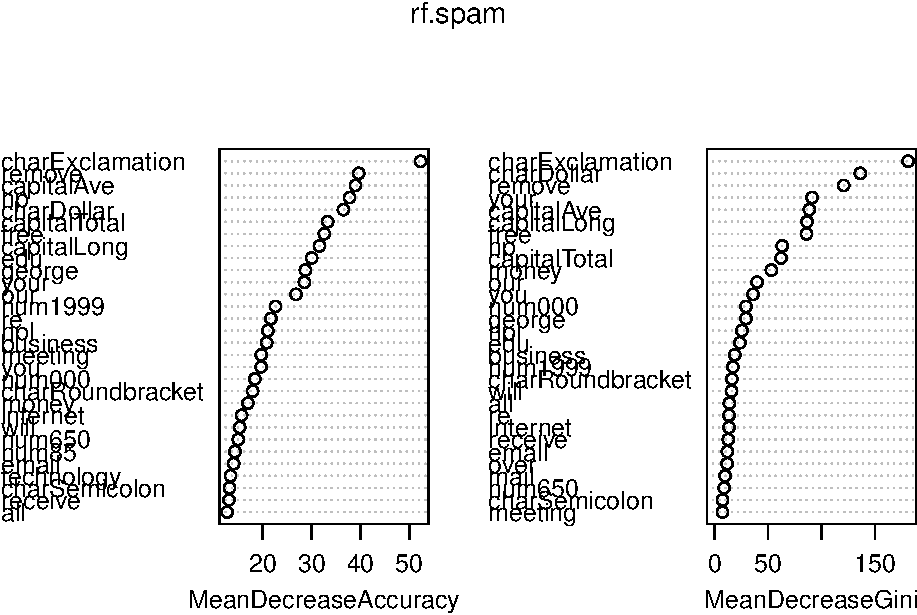
\includegraphics{8Trees_files/figure-beamer/unnamed-chunk-18-1.pdf}

\end{frame}

\begin{frame}[fragile]

\begin{Shaded}
\begin{Highlighting}[]
\KeywordTok{print}\NormalTok{(cv.headG)}
\end{Highlighting}
\end{Shaded}

\begin{verbatim}
## $size
##  [1] 75 26 21 18 16 12 10  7  6  4  1
## 
## $dev
##  [1] 129 129 129 129 129 129 131 131 149 149 166
## 
## $k
##  [1]       -Inf  0.0000000  0.2000000  0.3333333  0.5000000  0.7500000
##  [7]  1.0000000  2.0000000  6.0000000  6.5000000 11.0000000
## 
## $method
## [1] "misclass"
## 
## attr(,"class")
## [1] "prune"         "tree.sequence"
\end{verbatim}

\end{frame}

\begin{frame}

\begin{block}{Questions:}

Discuss the bias-variance tradeoff of a regression tree when
increasing/decreasing the number of terminal nodes, i.e:

\begin{itemize}
\tightlist
\item
  What happens to the bias?
\item
  What happens to the variance of a prediction if we reduce the tree
  size?
\end{itemize}

\end{block}

\end{frame}

\begin{frame}

\textbf{A}:

As the tree size increase the bias will decrease, and the variance will
increase. This is the same as any other method when we increase the
model complexity.

\end{frame}

\begin{frame}{From trees to forests}

\textbf{Advantages (+)}

\begin{itemize}
\tightlist
\item
  Trees automatically select variables
\item
  Tree-growing algorithms scale well to large \(n\), growing a tree
  greedily
\item
  Trees can handle mixed features (continouos, categorical) seamlessly,
  and can deal with missing data
\item
  Small trees are easy to interpret and explain to people
\item
  Some believe that decision trees mirror human decision making
\item
  Trees can be displayed graphically
\end{itemize}

\textbf{Disadvantages (-)}

\begin{itemize}
\tightlist
\item
  Large trees are not easy to interpret
\item
  Trees do not generally have good prediction performance (high
  variance)
\item
  Trees are not very robust, a small change in the data may cause a
  large change in the final estimated tree
\end{itemize}

\end{frame}

\begin{frame}

\begin{block}{What is next?}

\begin{itemize}
\tightlist
\item
  \textbf{Bagging}: grow many trees (from bootstrapped data) and average
  - to get rid of the non-robustness and high variance by averaging
\item
  Variable importance plot - to see which variables make a difference
  (now that we have many trees).
\item
  \textbf{Random forest}: inject more randomness (and even less
  variance) by just allowing a random selection of predictors to be used
  for the splits at each node.
\item
  \textbf{Boosting}: make one tree, then another based on the residuals
  from the previous, repeat. The final predictor is a weighted sum of
  these trees.
\end{itemize}

\end{block}

\end{frame}

\begin{frame}

But first,

\begin{block}{Leo Breiman - the inventor of CART, bagging and random
forests}

Quotation from
\href{https://en.wikipedia.org/wiki/Leo_Breiman}{Wikipedia}

Leo Breiman (January 27, 1928 -- July 5, 2005) was a distinguished
statistician at the University of California, Berkeley. He was the
recipient of numerous honors and awards, and was a member of the United
States National Academy of Science.

Breiman's work helped to bridge the gap between statistics and computer
science, particularly in the field of machine learning. His most
important contributions were his work on classification and regression
trees and ensembles of trees fit to bootstrap samples. Bootstrap
aggregation was given the name bagging by Breiman. Another of Breiman's
ensemble approaches is the random forest.

\end{block}

\end{frame}

\begin{frame}

From
\href{https://www.berkeley.edu/news/media/releases/2005/07/07_breiman.shtml}{Breimans
obituary}

BERKELEY -- Leo Breiman, professor emeritus of statistics at the
University of California, Berkeley.

``It is trite to say so, but Leo Breiman was indeed a Renaissance man,
and we shall miss him greatly,'' said Peter Bickel, professor of
statistics and chairman this summer of UC Berkeley's statistics
department.

Breiman retired in 1993, but as a Professor in the Graduate School, he
continued to get substantial National Science Foundation grants and
supervised three Ph.D.~students. Bickel said that some of Breiman's best
work was done after retirement.

\end{frame}

\begin{frame}

``In particular,'' said Bickel, ``he developed one of the most
successful state-of-the-art classification programs, `Random Forest.'
This method was based on a series of new ideas that he developed in
papers during the last seven years, and it is extensively used in
government and industry.''

Breiman's best known work is considered to be ``Classification and
Regression Trees,'' a work in collaboration with three other scholars
that facilitates practical applications, such as the diagnosis of
diseases, from a multitude of symptoms.

\end{frame}

\begin{frame}{Bagging}

Decision trees often suffer from high variance. By this we mean that the
trees are sensitive to small changes in the predictors: If we change the
observation set, we may get a very different tree.

Let's draw a new training set for our data and see what happens if we
fit our full classification tree (deviance grown).

\end{frame}

\begin{frame}[fragile]

\begin{Shaded}
\begin{Highlighting}[]
\KeywordTok{set.seed}\NormalTok{(}\DecValTok{33}\NormalTok{)}
\NormalTok{N =}\StringTok{ }\KeywordTok{dim}\NormalTok{(headInjury2)[}\DecValTok{1}\NormalTok{]}
\NormalTok{train2 =}\StringTok{ }\KeywordTok{sample}\NormalTok{(}\DecValTok{1}\OperatorTok{:}\NormalTok{N, }\DecValTok{850}\NormalTok{)  }\CommentTok{#We draw a new training sample. The number of observations is the same as before.}
\NormalTok{tree.HIClass2 =}\StringTok{ }\KeywordTok{tree}\NormalTok{(brain.injury }\OperatorTok{~}\StringTok{ }\NormalTok{., }\DataTypeTok{data =}\NormalTok{ headInjury2, }\DataTypeTok{subset =}\NormalTok{ train2)}
\KeywordTok{par}\NormalTok{(}\DataTypeTok{mfrow =} \KeywordTok{c}\NormalTok{(}\DecValTok{1}\NormalTok{, }\DecValTok{2}\NormalTok{))}
\CommentTok{# short=c('amnesia','bskullf','GCSdecr','GCS.13','GCS.15','risk','consc','oskullf','vomit','brain','age')}
\KeywordTok{plot}\NormalTok{(tree.HIClass)}
\KeywordTok{text}\NormalTok{(tree.HIClass, }\DataTypeTok{pretty =} \DecValTok{0}\NormalTok{)}
\KeywordTok{plot}\NormalTok{(tree.HIClass2)}
\KeywordTok{text}\NormalTok{(tree.HIClass2, }\DataTypeTok{pretty =} \DecValTok{0}\NormalTok{)}
\end{Highlighting}
\end{Shaded}

\includegraphics{8Trees_files/figure-beamer/unnamed-chunk-20-1.pdf}

\end{frame}

\begin{frame}

This classification tree is constructed by using \(850\) observations,
just like the tree in the \href{classtree2}{classification trees
section}, but we get two different trees that will give different
predictions for a test set.

To reduce the variance of decision trees we can apply \emph{bootstrap
aggregating} (\emph{bagging}), invented by Leo Breiman in 1996 (see
\href{ref}{references}).

\end{frame}

\begin{frame}

\begin{block}{Independent data sets}

Assume we have \(B\) i.i.d. observations of a random variable \(X\) each
with the same mean and with variance \(\sigma^2\). We calculate the mean
\(\bar{X} = \frac{1}{B} \sum_{b=1}^B X_b\). The variance of the mean is
\[\text{Var}(\bar{X}) = \text{Var}\Big(\frac{1}{B}\sum_{b=1}^B X_b \Big) = \frac{1}{B^2} \sum_{b=1}^B \text{Var}(X_b) = \frac{\sigma^2}{B}.\]
By averaging we get reduced variance. This is the basic idea!

But, we will not draw random variables - we want to fit decision trees:
\(\hat{f}_1({\bf x}),\hat{f}_2({\bf x}),\ldots, \hat{f}_B({\bf x})\) and
average those.
\[ \hat{f}_{avg}({\bf x})=\frac{1}{B}\sum_{b=1}^B \hat{f}_b({\bf x})\]

However, we do not have many independent data set - so we use
\emph{bootstrapping} to construct \(B\) data sets.

\end{block}

\end{frame}

\begin{frame}

\begin{block}{Bootstrapping (from Module 5)}

Problem: we want to draw samples from a population with distribution
\(f\).

But: we do not know \(f\) and do not have a population to draw from, we
only have our one sample.

Solution: we may use our sample as an empirical estimate for the
distribution \(f\) - by assuming that each sample point has probability
\(1/n\) for being drawn.

Therefore: we draw with replacement \(n\) observations from our sample -
and that is our first \emph{bootstrap sample}.

We repeat this \(B\) times and get \(B\) bootstrap samples - that we use
as our \(B\) data sets.

\end{block}

\end{frame}

\begin{frame}

\begin{block}{Bootstrap samples and trees}

For each bootstrap sample we construct a decision tree,
\(\hat{f}^{*b}(x)\) with \(b=1,...,B\), and we then use information from
all of the trees to draw inference.

For a regression tree, we take the average of all of the predictions and
use this as the final result: \[
\hat{f}_{bag}(x)=\frac{1}{B}\sum_{b=1}^B \hat{f}^{*b}(x).
\] For a classification tree we record the predicted class (for a given
observation \(x\)) for each of the \(B\) trees and use the most
occurring classification (majority vote) as the final prediction - or
alternatively average posterior probabilities for each class.

\end{block}

\end{frame}

\begin{frame}

Originally, Breiman (1996) suggested to prune each tree, but later
research has found that it is better to leave the trees at maximal size
(a bushy tree), to make the trees as different from each other as
possible.

The number \(B\) is chosen to be as large as ``necessary''. An increase
in \(B\) will not lead to overfitting, and \(B\) is not regarded as a
tuning parameter. If a goodness of fit measure is plotted as a function
of \(B\) (soon) we see that (given that \(B\) is large enough)
increasing \(B\) will not change the goodness of fit measure.

But first, a smart way to avoid doing cross-validation.

\end{frame}

\begin{frame}

\begin{block}{Out-of-bag error estimation}

\begin{itemize}
\tightlist
\item
  We use a subset of the observations in each bootstrap sample. From
  Module 5 we know that the probability that an observation is in the
  bootstrap sample is approximately \(1-e^{-1}\)=0.6321206
  (approximately 2/3).
\item
  when an observation is left out of the bootstrap sample it is not used
  to build the tree, and we can use this observation as a part of a
  ``test set'' to measure the predictive performance and error of the
  fitted model, \(f^{*b}(x)\).
\end{itemize}

In other words: Since each observation \(i\) has a probability of
approximately 2/3 to be in a bootstrap sample, and we make \(B\)
bootstrap samples, then observation \(i\) will be outside the bootstrap
sample in approximately \(B/3\) of the fitted trees.

The observations left out are referred to as the \emph{out-of-bag}
observations, and the measured error of the \(B/3\) predictions is
called the \emph{out-of-bag error}.

\end{block}

\end{frame}

\begin{frame}[fragile]

\begin{block}{Example}

We can do bagging by using the function \emph{randomForest()} in the
\emph{randomForest} library.

\footnotesize

\begin{Shaded}
\begin{Highlighting}[]
\KeywordTok{library}\NormalTok{(randomForest)}
\KeywordTok{set.seed}\NormalTok{(}\DecValTok{1}\NormalTok{)}
\NormalTok{bag =}\StringTok{ }\KeywordTok{randomForest}\NormalTok{(brain.injury }\OperatorTok{~}\StringTok{ }\NormalTok{., }\DataTypeTok{data =}\NormalTok{ headInjury2, }\DataTypeTok{subset =}\NormalTok{ train, }
    \DataTypeTok{mtry =} \DecValTok{10}\NormalTok{, }\DataTypeTok{ntree =} \DecValTok{500}\NormalTok{, }\DataTypeTok{importance =} \OtherTok{TRUE}\NormalTok{)}
\NormalTok{bag}\OperatorTok{$}\NormalTok{confusion}
\end{Highlighting}
\end{Shaded}

\begin{verbatim}
##     0  1 class.error
## 0 637 54  0.07814761
## 1  76 83  0.47798742
\end{verbatim}

\begin{Shaded}
\begin{Highlighting}[]
\DecValTok{1} \OperatorTok{-}\StringTok{ }\KeywordTok{sum}\NormalTok{(}\KeywordTok{diag}\NormalTok{(bag}\OperatorTok{$}\NormalTok{confusion))}\OperatorTok{/}\KeywordTok{sum}\NormalTok{(bag}\OperatorTok{$}\NormalTok{confusion[}\DecValTok{1}\OperatorTok{:}\DecValTok{2}\NormalTok{, }\DecValTok{1}\OperatorTok{:}\DecValTok{2}\NormalTok{])}
\end{Highlighting}
\end{Shaded}

\begin{verbatim}
## [1] 0.1529412
\end{verbatim}

\normalsize

The variable \emph{mtry=10} because we want to consider all \(10\)
predictors in each split of the tree. The variable \(ntree=500\) because
we want to average over \(500\) trees.

\end{block}

\end{frame}

\begin{frame}[fragile]

Predictive performance of the bagged tree on unseen test data:

\begin{Shaded}
\begin{Highlighting}[]
\NormalTok{yhat.bag =}\StringTok{ }\KeywordTok{predict}\NormalTok{(bag, }\DataTypeTok{newdata =}\NormalTok{ headInjury2[test, ])}
\NormalTok{misclass.bag =}\StringTok{ }\KeywordTok{table}\NormalTok{(yhat.bag, headInjury2[test, ]}\OperatorTok{$}\NormalTok{brain.injury)}
\KeywordTok{print}\NormalTok{(misclass.bag)}
\end{Highlighting}
\end{Shaded}

\begin{verbatim}
##         
## yhat.bag   0   1
##        0 346  39
##        1  34  52
\end{verbatim}

\begin{Shaded}
\begin{Highlighting}[]
\DecValTok{1} \OperatorTok{-}\StringTok{ }\KeywordTok{sum}\NormalTok{(}\KeywordTok{diag}\NormalTok{(misclass.bag))}\OperatorTok{/}\NormalTok{(}\KeywordTok{sum}\NormalTok{(misclass.bag))}
\end{Highlighting}
\end{Shaded}

\begin{verbatim}
## [1] 0.1549894
\end{verbatim}

We note that the misclassification rate has increased slightly for the
bagged tree (as compared to our previous full and pruned tree).
\textbf{In other examples an improvement is very often seen.}

\end{frame}

\begin{frame}

\begin{block}{Prediction by majority vote vs.~by averaging the
probabilities}

Consider the case when you have grown \(B\) classification tree with a
binary response with classes 0 and 1. You might wonder which approach to
choose to make a final prediction: majority vote or an average of the
probabilities? Or would the prediction be the same in each case?

The difference between these two procedures can be compared to the
difference between the mean value and median of a set of numbers. If we
average the probabilities and make a classification thereafter, we have
the mean value. If we sort all of our classifications, so that the
classifications corresponding to one class would be lined up after each
other, followed by the classifications corresponding to the other class
we obtain the median value.

\end{block}

\end{frame}

\begin{frame}

We examine this by an example:

Suppose we have \(B=5\) (no, \(B\) should be higher - this is only for
illustration) classification tree and have obtained the following 5
estimated probabilities: \{0.4, 0.4, 0.4, 0.4, 0.9 \}. If we average the
probabilities, we get 0.5, and if we use a cut-off value of 0.5, our
predicted class is 1. However, if we take a majority vote, using the
same cut of value, the predicted classes will be \{0, 0, 0, 0, 1 \}. The
predicted class, based on a majority vote, would accordingly be 0.

The two procedures thus have their pros and cons: By averaging the
predictions no information is lost. We do not only get the final
classification, but the probability for belonging to the class 0 or 1.
However, this method is not robust to outliers. By taking a majority
vote, outliers have a smaller influence on the result.

\end{frame}

\begin{frame}

\begin{block}{When should we use bagging?}

Bagging can be used for predictors (regression and classification) that
are not trees, and according to Breiman (1996)

\begin{itemize}
\tightlist
\item
  the vital element is the instability of the prediction method
\item
  if perturbing the learning set can cause significant changes in the
  predictor constructed, then bagging can improve accuracy.
\end{itemize}

Breiman (1996) suggests that these methods should be suitable for
bagging:

\begin{itemize}
\tightlist
\item
  neural nets, classification and regression trees, subset selection in
  linear regression
\end{itemize}

however not nearest neigbours - since

\begin{itemize}
\tightlist
\item
  the stability of nearest neighbour classification methods with respect
  to perturbations of the data distinguishes them from competitors such
  as trees and neural nets.
\end{itemize}

\end{block}

\end{frame}

\begin{frame}

\begin{block}{Variable importance plots}

Bagging is an example of an \emph{ensemble method}, so is boosting and
random forests (to come next). For all of these methods many trees are
grown and combined, and the predictive power can be highly improved.
However, this comes at a cost of interpretability. Instead of having one
tree, the resulting model consists of \(B\) trees, where \(B\) often is
300 or 500 (or maybe even 5000 when boosting).

Variable importance plots show \emph{the relative importance of the
predictors:} the predictors are sorted according to their importance,
such that the top variables have a higher importance than the bottom
variables. There are in general two types of variable importance plots:

\begin{itemize}
\tightlist
\item
  variable importance based on decrease in node impurity and
\item
  variable importance based on randomization.
\end{itemize}

\end{block}

\end{frame}

\begin{frame}

\begin{block}{Variable importance based on node impurity}

The term \emph{important} relates to \emph{total decrease in the node
impurity, over splits for a predictor}, and is defined differently for
regression trees and classification trees.

\textbf{Regression trees:}

\begin{itemize}
\tightlist
\item
  The importance of each predictor is calculated using the RSS.
\item
  The algorithm records the total amount that the RSS is decreased due
  to splits for each predictor (there may be many spits for one
  predictor for each tree).
\item
  This decrease in RSS is then averaged over the \(B\) trees. The higher
  the decrease, the more important the predictor.
\end{itemize}

\end{block}

\end{frame}

\begin{frame}[fragile]

\textbf{Classification trees:}

\begin{itemize}
\tightlist
\item
  The importance of each predictor is calculated using the Gini index.
\item
  The importance is the mean decrease (over all \(B\) trees) in the Gini
  index by splits of a predictor.
\end{itemize}

R: \texttt{varImpPlot} (or \texttt{importance}) in \texttt{randomForest}
with \texttt{type=2}.

\end{frame}

\begin{frame}[fragile]

\textbf{Auto data example}

\begin{Shaded}
\begin{Highlighting}[]
\KeywordTok{set.seed}\NormalTok{(}\DecValTok{4268}\NormalTok{)}
\KeywordTok{data}\NormalTok{(mtcars)}
\NormalTok{mtcars.rf <-}\StringTok{ }\KeywordTok{randomForest}\NormalTok{(mpg }\OperatorTok{~}\StringTok{ }\NormalTok{., }\DataTypeTok{data =}\NormalTok{ mtcars, }\DataTypeTok{ntree =} \DecValTok{1000}\NormalTok{, }\DataTypeTok{keep.forest =} \OtherTok{FALSE}\NormalTok{, }
    \DataTypeTok{importance =} \OtherTok{TRUE}\NormalTok{)}
\end{Highlighting}
\end{Shaded}

\end{frame}

\begin{frame}[fragile]

\begin{Shaded}
\begin{Highlighting}[]
\KeywordTok{varImpPlot}\NormalTok{(mtcars.rf, }\DataTypeTok{type =} \DecValTok{2}\NormalTok{, }\DataTypeTok{pch =} \DecValTok{20}\NormalTok{)}
\end{Highlighting}
\end{Shaded}

\includegraphics{8Trees_files/figure-beamer/unnamed-chunk-24-1.pdf}

\end{frame}

\begin{frame}[fragile]

\begin{block}{Variable importance based on randomization}

Variable importance based on randomization is calculated using the OOB
sample.

\begin{itemize}
\tightlist
\item
  Computations are carried out for one bootstrap sample at a time.
\item
  Each time a tree is grown the OOB sample is used to test the
  predictive power of the tree.
\item
  Then for one predictor at a time, repeat the following:

  \begin{itemize}
  \tightlist
  \item
    permute the OOB observations for the \(j\)th variable \(x_j\) and
    calculate the new OOB error.
  \item
    If \(x_j\) is important, permuting its observations will decrease
    the predictive performance.
  \end{itemize}
\item
  The difference between the two is averaged over all trees (and
  normalized by the standard deviation of the differences).
\end{itemize}

R: \texttt{varImpPlot} (or \texttt{importance}) in \texttt{randomForest}
with \texttt{type=1}.

\end{block}

\end{frame}

\begin{frame}[fragile]

\begin{Shaded}
\begin{Highlighting}[]
\KeywordTok{varImpPlot}\NormalTok{(mtcars.rf, }\DataTypeTok{type =} \DecValTok{1}\NormalTok{, }\DataTypeTok{pch =} \DecValTok{20}\NormalTok{)}
\end{Highlighting}
\end{Shaded}

\includegraphics{8Trees_files/figure-beamer/unnamed-chunk-25-1.pdf}

\end{frame}

\begin{frame}[fragile]

The two types together: do they agree?

\begin{Shaded}
\begin{Highlighting}[]
\KeywordTok{varImpPlot}\NormalTok{(mtcars.rf, }\DataTypeTok{pch =} \DecValTok{20}\NormalTok{)}
\end{Highlighting}
\end{Shaded}

\includegraphics{8Trees_files/figure-beamer/unnamed-chunk-26-1.pdf}

\end{frame}

\begin{frame}{Random Forest}

If there is a strong predictor in the dataset, the decision trees
produced by each of the bootstrap samples in the bagging algorithm
becomes very similar: Most of the trees will use the same strong
predictor in the top split.

We have seen this for our example trees for the minor head injury
example, the predictor \emph{GCS.15.2hours} was chosen in the top split
every time. This is probably the case for a large amount of the bagged
trees as well.

This is not optimal, because we get \(B\) trees that are highly
correlated. We don't get a large reduction in variance by averaging
\(\hat{f}^{*b}(x)\) when the correlation between the trees is high. In
the \href{bagex}{previous section} we actually saw a (marginal) decrease
in the predictive performance for the bagged tree compared to the
\href{expruning}{pruned tree} and the \href{classtree2}{full tree}.

\emph{Random forests} is a solution to this problem and a method for
decorrelating the trees.

\end{frame}

\begin{frame}

\begin{block}{The effect of correlation on the variance of the mean}

The variance of the average of \(B\) observations of i.i.d random
variables \(X\), each with variance \(\sigma^2\) is
\(\frac{\sigma^2}{B}\). Now, suppose we have \(B\) observations of a
random variable \(X\) which are identically distributed, each with mean
\(\mu\) and variance \(\sigma^2\), but not independent.

That is, suppose the variables have a positive correlation \(\rho\)
\[\text{Cov}(X_i, X_j) = \rho \sigma^2, \quad i \neq j.\]

\end{block}

\end{frame}

\begin{frame}

The variance of the average is
\[\begin{aligned} \text{Var}(\bar{X}) &= \text{Var}\Big( \frac{1}{B}\sum_{i=1}^B X_i \Big) \\
&= \sum_{i=1}^B \frac{1}{B^2} \text{Var} (X_i) + 2 \sum_{i=2}^B \sum_{j=1}^{i-1} \frac{1}{B} \frac{1}{B} \text{Cov} (X_i, X_j) \\
&= \frac{1}{B} \sigma^2 + 2 \frac{B(B-1)}{2}\frac{1}{B^2} \rho \sigma^2 \\
&= \frac{1}{B} \sigma^2 + \rho \sigma^2 - \frac{1}{B} \rho \sigma^2 \\
&= \rho \sigma^2 + \frac{1-\rho}{B}\sigma^2\\
&= \frac{1-(1-B)\rho}{B} \sigma^2\\ \end{aligned}\]

Check: \(\rho=0\) and \(\rho=1\)? (Most negative values of \(\rho\) will
not give a positive definite covariance matrix. The covariance matrix is
positive definite if \(\rho>-1/(B-1)\).)

\end{frame}

\begin{frame}

The idea behind random forests is to \emph{improve the variance
reduction of bagging} by reducing the correlation between the trees.

The procedure is thus as in bagging, but with the important difference,
that

\begin{itemize}
\tightlist
\item
  at each split we are only allowed to consider \(m<p\) of the
  predictors.
\end{itemize}

A new sample of \(m\) predictors is taken at each split and

\begin{itemize}
\tightlist
\item
  typically \(m\approx \sqrt p\) (classificaton) and \(m=p/3\)
  (regression)
\end{itemize}

The general idea is at for very correlated predictors \(m\) is chosen to
be small.

\end{frame}

\begin{frame}

The number of trees, \(B\), is not a tuning parameter, and the best is
to choose it large enough.

If \(B\) is sufficiently large (three times the number needed for the
random forest to stabilize), the OOB error estimate is equvalent to
LOOCV (Efron and Hastie, 2016, p 330).

\end{frame}

\begin{frame}

\includegraphics{../../ISLR/Figures/Chapter8/8.10.png}

\end{frame}

\begin{frame}[fragile]

\begin{block}{Example}

We decorrelate the trees by using the \emph{randomForest()} function
again, but this time we set \emph{mtry=3}. This means that the algorithm
only considers three of the predictors in each split. We choose \(3\)
because we have \(10\) predictors in total and \(\sqrt{10}\approx 3\).

\begin{Shaded}
\begin{Highlighting}[]
\KeywordTok{set.seed}\NormalTok{(}\DecValTok{1}\NormalTok{)}

\NormalTok{rf =}\StringTok{ }\KeywordTok{randomForest}\NormalTok{(brain.injury }\OperatorTok{~}\StringTok{ }\NormalTok{., }\DataTypeTok{data =}\NormalTok{ headInjury2, }\DataTypeTok{subset =}\NormalTok{ train, }
    \DataTypeTok{mtry =} \DecValTok{3}\NormalTok{, }\DataTypeTok{ntree =} \DecValTok{500}\NormalTok{, }\DataTypeTok{importance =} \OtherTok{TRUE}\NormalTok{)}
\end{Highlighting}
\end{Shaded}

\end{block}

\end{frame}

\begin{frame}[fragile]

We check the predictive performance as before: \footnotesize

\begin{Shaded}
\begin{Highlighting}[]
\NormalTok{rf}\OperatorTok{$}\NormalTok{confusion}
\end{Highlighting}
\end{Shaded}

\begin{verbatim}
##     0  1 class.error
## 0 662 29  0.04196816
## 1  93 66  0.58490566
\end{verbatim}

\begin{Shaded}
\begin{Highlighting}[]
\DecValTok{1} \OperatorTok{-}\StringTok{ }\KeywordTok{sum}\NormalTok{(}\KeywordTok{diag}\NormalTok{(rf}\OperatorTok{$}\NormalTok{confusion[}\DecValTok{1}\OperatorTok{:}\DecValTok{2}\NormalTok{, }\DecValTok{1}\OperatorTok{:}\DecValTok{2}\NormalTok{]))}\OperatorTok{/}\NormalTok{(}\KeywordTok{sum}\NormalTok{(rf}\OperatorTok{$}\NormalTok{confusion[}\DecValTok{1}\OperatorTok{:}\DecValTok{2}\NormalTok{, }\DecValTok{1}\OperatorTok{:}\DecValTok{2}\NormalTok{]))}
\end{Highlighting}
\end{Shaded}

\begin{verbatim}
## [1] 0.1435294
\end{verbatim}

\begin{Shaded}
\begin{Highlighting}[]
\NormalTok{yhat.rf =}\StringTok{ }\KeywordTok{predict}\NormalTok{(rf, }\DataTypeTok{newdata =}\NormalTok{ headInjury2[test, ])}

\NormalTok{misclass.rf =}\StringTok{ }\KeywordTok{table}\NormalTok{(yhat.rf, headInjury2[test, ]}\OperatorTok{$}\NormalTok{brain.injury)}
\KeywordTok{print}\NormalTok{(misclass.rf)}
\end{Highlighting}
\end{Shaded}

\begin{verbatim}
##        
## yhat.rf   0   1
##       0 364  47
##       1  16  44
\end{verbatim}

\begin{Shaded}
\begin{Highlighting}[]
\DecValTok{1} \OperatorTok{-}\StringTok{ }\KeywordTok{sum}\NormalTok{(}\KeywordTok{diag}\NormalTok{(misclass.rf))}\OperatorTok{/}\NormalTok{(}\KeywordTok{sum}\NormalTok{(misclass.rf))}
\end{Highlighting}
\end{Shaded}

\begin{verbatim}
## [1] 0.133758
\end{verbatim}

\normalsize

The misclassification rate is slightly decreased compared to the
\href{bagex}{bagged tree} (and to the \href{expruning}{pruned tree}).

\end{frame}

\begin{frame}[fragile]

By using the \emph{varImpPlot()} function we can study the importance of
each predictor.

\begin{Shaded}
\begin{Highlighting}[]
\KeywordTok{varImpPlot}\NormalTok{(rf, }\DataTypeTok{pch =} \DecValTok{20}\NormalTok{)}
\end{Highlighting}
\end{Shaded}

\includegraphics{8Trees_files/figure-beamer/unnamed-chunk-30-1.pdf}

\begin{Shaded}
\begin{Highlighting}[]
\KeywordTok{varImpPlot}\NormalTok{(rf, }\DataTypeTok{pch =} \DecValTok{20}\NormalTok{, }\DataTypeTok{type =} \DecValTok{1}\NormalTok{)}
\end{Highlighting}
\end{Shaded}

\includegraphics{8Trees_files/figure-beamer/unnamed-chunk-30-2.pdf}

\begin{Shaded}
\begin{Highlighting}[]
\KeywordTok{varImpPlot}\NormalTok{(rf, }\DataTypeTok{pch =} \DecValTok{20}\NormalTok{, }\DataTypeTok{type =} \DecValTok{2}\NormalTok{)}
\end{Highlighting}
\end{Shaded}

\includegraphics{8Trees_files/figure-beamer/unnamed-chunk-30-3.pdf}

As expected \emph{GCS.15.2hours} is a strong predictor along with
\emph{basal.skull.facture} and \emph{age}. This means that most of the
trees will have these predictors in the top split.

\end{frame}

\begin{frame}[fragile]

\textbf{Iris example}

Variable importance plot for bagging:

\begin{Shaded}
\begin{Highlighting}[]
\CommentTok{# borrowed from}
\CommentTok{# https://gist.github.com/ramhiser/6dec3067f087627a7a85}
\KeywordTok{library}\NormalTok{(dplyr)}
\KeywordTok{library}\NormalTok{(ggplot2)}
\CommentTok{# library(ggpubr)}
\NormalTok{rf_out <-}\StringTok{ }\KeywordTok{randomForest}\NormalTok{(Species }\OperatorTok{~}\StringTok{ }\NormalTok{., }\DataTypeTok{data =}\NormalTok{ iris, }\DataTypeTok{mtry =} \DecValTok{4}\NormalTok{)}
\NormalTok{rf_out}\OperatorTok{$}\NormalTok{confusion}
\end{Highlighting}
\end{Shaded}

\begin{verbatim}
##            setosa versicolor virginica class.error
## setosa         50          0         0        0.00
## versicolor      0         47         3        0.06
## virginica       0          3        47        0.06
\end{verbatim}

\begin{Shaded}
\begin{Highlighting}[]
\CommentTok{# Extracts variable importance (Mean Decrease in Gini Index) Sorts}
\CommentTok{# by variable importance and relevels factors to match ordering}
\NormalTok{var_importance <-}\StringTok{ }\KeywordTok{data_frame}\NormalTok{(}\DataTypeTok{variable =} \KeywordTok{setdiff}\NormalTok{(}\KeywordTok{colnames}\NormalTok{(iris), }\StringTok{"Species"}\NormalTok{), }
    \DataTypeTok{importance =} \KeywordTok{as.vector}\NormalTok{(}\KeywordTok{importance}\NormalTok{(rf_out)))}
\NormalTok{var_importance <-}\StringTok{ }\KeywordTok{arrange}\NormalTok{(var_importance, }\KeywordTok{desc}\NormalTok{(importance))}
\NormalTok{var_importance}\OperatorTok{$}\NormalTok{variable <-}\StringTok{ }\KeywordTok{factor}\NormalTok{(var_importance}\OperatorTok{$}\NormalTok{variable, }\DataTypeTok{levels =}\NormalTok{ var_importance}\OperatorTok{$}\NormalTok{variable)}

\NormalTok{p <-}\StringTok{ }\KeywordTok{ggplot}\NormalTok{(var_importance, }\KeywordTok{aes}\NormalTok{(}\DataTypeTok{x =}\NormalTok{ variable, }\DataTypeTok{weight =}\NormalTok{ importance, }
    \DataTypeTok{fill =}\NormalTok{ variable))}
\NormalTok{p <-}\StringTok{ }\NormalTok{p }\OperatorTok{+}\StringTok{ }\KeywordTok{geom_bar}\NormalTok{() }\OperatorTok{+}\StringTok{ }\KeywordTok{ggtitle}\NormalTok{(}\StringTok{"Variable Importance from Random Forest Fit"}\NormalTok{)}
\NormalTok{p <-}\StringTok{ }\NormalTok{p }\OperatorTok{+}\StringTok{ }\KeywordTok{xlab}\NormalTok{(}\StringTok{"Demographic Attribute"}\NormalTok{) }\OperatorTok{+}\StringTok{ }\KeywordTok{ylab}\NormalTok{(}\StringTok{"Variable Importance (Mean Decrease in Gini Index)"}\NormalTok{)}
\NormalTok{p <-}\StringTok{ }\NormalTok{p }\OperatorTok{+}\StringTok{ }\KeywordTok{scale_fill_discrete}\NormalTok{(}\DataTypeTok{name =} \StringTok{"Variable Name"}\NormalTok{)}
\NormalTok{p =}\StringTok{ }\NormalTok{p }\OperatorTok{+}\StringTok{ }\KeywordTok{theme}\NormalTok{(}\DataTypeTok{axis.text.x =} \KeywordTok{element_blank}\NormalTok{(), }\DataTypeTok{axis.text.y =} \KeywordTok{element_text}\NormalTok{(}\DataTypeTok{size =} \DecValTok{12}\NormalTok{), }
    \DataTypeTok{axis.title =} \KeywordTok{element_text}\NormalTok{(}\DataTypeTok{size =} \DecValTok{16}\NormalTok{), }\DataTypeTok{plot.title =} \KeywordTok{element_text}\NormalTok{(}\DataTypeTok{size =} \DecValTok{18}\NormalTok{), }
    \DataTypeTok{legend.title =} \KeywordTok{element_text}\NormalTok{(}\DataTypeTok{size =} \DecValTok{16}\NormalTok{), }\DataTypeTok{legend.text =} \KeywordTok{element_text}\NormalTok{(}\DataTypeTok{size =} \DecValTok{12}\NormalTok{))}
\NormalTok{p}
\end{Highlighting}
\end{Shaded}

\includegraphics{8Trees_files/figure-beamer/unnamed-chunk-31-1.pdf}

\end{frame}

\begin{frame}[fragile]

\textbf{Iris example}

Variable importance plot for random forest:

\begin{Shaded}
\begin{Highlighting}[]
\CommentTok{# borrowed from}
\CommentTok{# https://gist.github.com/ramhiser/6dec3067f087627a7a85}

\NormalTok{rf_out =}\StringTok{ }\KeywordTok{randomForest}\NormalTok{(Species }\OperatorTok{~}\StringTok{ }\NormalTok{., }\DataTypeTok{data =}\NormalTok{ iris)}
\NormalTok{rf_out}\OperatorTok{$}\NormalTok{confusion}
\end{Highlighting}
\end{Shaded}

\begin{verbatim}
##            setosa versicolor virginica class.error
## setosa         50          0         0        0.00
## versicolor      0         47         3        0.06
## virginica       0          4        46        0.08
\end{verbatim}

\begin{Shaded}
\begin{Highlighting}[]
\NormalTok{var_importance <-}\StringTok{ }\KeywordTok{data_frame}\NormalTok{(}\DataTypeTok{variable =} \KeywordTok{setdiff}\NormalTok{(}\KeywordTok{colnames}\NormalTok{(iris), }\StringTok{"Species"}\NormalTok{), }
    \DataTypeTok{importance =} \KeywordTok{as.vector}\NormalTok{(}\KeywordTok{importance}\NormalTok{(rf_out)))}
\NormalTok{var_importance <-}\StringTok{ }\KeywordTok{arrange}\NormalTok{(var_importance, }\KeywordTok{desc}\NormalTok{(importance))}
\NormalTok{var_importance}\OperatorTok{$}\NormalTok{variable <-}\StringTok{ }\KeywordTok{factor}\NormalTok{(var_importance}\OperatorTok{$}\NormalTok{variable, }\DataTypeTok{levels =}\NormalTok{ var_importance}\OperatorTok{$}\NormalTok{variable)}

\NormalTok{pp <-}\StringTok{ }\KeywordTok{ggplot}\NormalTok{(var_importance, }\KeywordTok{aes}\NormalTok{(}\DataTypeTok{x =}\NormalTok{ variable, }\DataTypeTok{weight =}\NormalTok{ importance, }
    \DataTypeTok{fill =}\NormalTok{ variable))}
\NormalTok{pp <-}\StringTok{ }\NormalTok{pp }\OperatorTok{+}\StringTok{ }\KeywordTok{geom_bar}\NormalTok{() }\OperatorTok{+}\StringTok{ }\KeywordTok{ggtitle}\NormalTok{(}\StringTok{"Variable Importance from Random Forest Fit"}\NormalTok{)}
\NormalTok{pp <-}\StringTok{ }\NormalTok{pp }\OperatorTok{+}\StringTok{ }\KeywordTok{xlab}\NormalTok{(}\StringTok{"Demographic Attribute"}\NormalTok{) }\OperatorTok{+}\StringTok{ }\KeywordTok{ylab}\NormalTok{(}\StringTok{"Variable Importance (Mean Decrease in Gini Index)"}\NormalTok{)}
\NormalTok{pp <-}\StringTok{ }\NormalTok{pp }\OperatorTok{+}\StringTok{ }\KeywordTok{scale_fill_discrete}\NormalTok{(}\DataTypeTok{name =} \StringTok{"Variable Name"}\NormalTok{)}
\NormalTok{pp =}\StringTok{ }\NormalTok{pp }\OperatorTok{+}\StringTok{ }\KeywordTok{theme}\NormalTok{(}\DataTypeTok{axis.text.x =} \KeywordTok{element_blank}\NormalTok{(), }\DataTypeTok{axis.text.y =} \KeywordTok{element_text}\NormalTok{(}\DataTypeTok{size =} \DecValTok{12}\NormalTok{), }
    \DataTypeTok{axis.title =} \KeywordTok{element_text}\NormalTok{(}\DataTypeTok{size =} \DecValTok{16}\NormalTok{), }\DataTypeTok{plot.title =} \KeywordTok{element_text}\NormalTok{(}\DataTypeTok{size =} \DecValTok{18}\NormalTok{), }
    \DataTypeTok{legend.title =} \KeywordTok{element_text}\NormalTok{(}\DataTypeTok{size =} \DecValTok{16}\NormalTok{), }\DataTypeTok{legend.text =} \KeywordTok{element_text}\NormalTok{(}\DataTypeTok{size =} \DecValTok{12}\NormalTok{))}
\NormalTok{pp}
\end{Highlighting}
\end{Shaded}

\includegraphics{8Trees_files/figure-beamer/unnamed-chunk-32-1.pdf}

\end{frame}

\begin{frame}{Boosting}

\emph{Boosting} is an alternative approach for improving the predictions
resulting from a decision tree. We will only consider the description of
boosting regression trees (and not classification trees) in this course.

In boosting the trees are grown \emph{sequentially} so that each tree is
grown using information from the previous tree.

\begin{itemize}
\tightlist
\item
  First build a decision tree with \(d\) splits (and \(d+1\) terminal
  notes).
\item
  Next, improve the model in areas where the model didn't perform well.
  This is done by fitting a decision tree to the \emph{residuals of the
  model}. This procedure is called \emph{learning slowly}.
\item
  The first decision tree is then updated based on the residual tree,
  but with a weight.
\item
  The procedure is repeated until some stopping criterion is reached.
  Each of the trees can be very small, with just a few terminal nodes
  (or just one split).
\end{itemize}

\end{frame}

\begin{frame}

\textbf{Algorithm 8.2: Boosting for regression trees}

\begin{enumerate}
\def\labelenumi{\arabic{enumi}.}
\tightlist
\item
  Set \(\hat{f}(x) = 0\) and \(r_i = y_i\) for all \(i\) in the training
  set.
\item
  For \(b=1,2,...,B\), repeat:

  \begin{enumerate}
  \def\labelenumii{\alph{enumii})}
  \tightlist
  \item
    Fit a tree \(\hat{f}^b\) with \(d\) splits (\(d+1\) terminal nodes)
    to the training data.\\
  \item
    Update \(\hat{f}\) by adding in a shrunken version of the new tree:
    \[\hat{f}(x) \leftarrow \hat{f}(x)+\lambda \hat{f}^b(x).\]\\
  \item
    Update the residuals,
    \[r_i \leftarrow r_i - \lambda \hat{f}^b(x_i).\]\\
  \end{enumerate}
\item
  The boosted model is
  \(\hat{f}(x) = \sum_{b=1}^B \lambda \hat{f}^b(x).\)
\end{enumerate}

Boosting has three tuning parameters which need to set, and can be found
using cross-validation.

\end{frame}

\begin{frame}

\textbf{Tuning parameters}

\begin{itemize}
\tightlist
\item
  The number of trees to be grown, \(B\). The value of \(B\) could be
  chosen using cross-validation. A too small value of \(B\) would imply
  that much information is unused (remember that boosting is a slow
  learner), whereas a too large value of \(B\) may lead to overfitting.
\item
  \(\lambda\): This is a shrinkage parameter and controls the rate at
  which boosting learns. The role of \(\lambda\) is to scale the new
  information, when added to the existing tree. We add information from
  the \(b\)-th tree to our existing tree \(\hat{f}\), but scaled by the
  \(\lambda\). Choosing a small value for \(\lambda\) ensures that the
  algorithm learns slowly, but will require a larger tree ensemble.
  Typical values of \(\lambda\) is 0.1 or 0.01.
\item
  Interaction depth \(d\): The number of splits in each tree. This
  parameter controls the complexity of the boosted tree ensemble (the
  level of interaction between variables that we may estimate). By
  choosing \(d=1\) a tree stump will be fitted at each step and this
  gives an additive model.
\end{itemize}

\end{frame}

\begin{frame}[fragile]{Example: Boston data set}

First - to get to know the data set we run through trees, bagging and
random forests - before arriving at boosting. See also the ISLR book,
Section 8.3.4.

\begin{block}{Data}

\begin{Shaded}
\begin{Highlighting}[]
\KeywordTok{library}\NormalTok{(MASS)}
\KeywordTok{library}\NormalTok{(tree)}
\KeywordTok{set.seed}\NormalTok{(}\DecValTok{1}\NormalTok{)}
\NormalTok{train =}\StringTok{ }\KeywordTok{sample}\NormalTok{(}\DecValTok{1}\OperatorTok{:}\KeywordTok{nrow}\NormalTok{(Boston), }\KeywordTok{nrow}\NormalTok{(Boston)}\OperatorTok{/}\DecValTok{2}\NormalTok{)}
\KeywordTok{colnames}\NormalTok{(Boston)}
\end{Highlighting}
\end{Shaded}

\begin{verbatim}
##  [1] "crim"    "zn"      "indus"   "chas"    "nox"     "rm"      "age"    
##  [8] "dis"     "rad"     "tax"     "ptratio" "black"   "lstat"   "medv"
\end{verbatim}

\begin{Shaded}
\begin{Highlighting}[]
\KeywordTok{head}\NormalTok{(Boston)}
\end{Highlighting}
\end{Shaded}

\begin{verbatim}
##      crim zn indus chas   nox    rm  age    dis rad tax ptratio  black
## 1 0.00632 18  2.31    0 0.538 6.575 65.2 4.0900   1 296    15.3 396.90
## 2 0.02731  0  7.07    0 0.469 6.421 78.9 4.9671   2 242    17.8 396.90
## 3 0.02729  0  7.07    0 0.469 7.185 61.1 4.9671   2 242    17.8 392.83
## 4 0.03237  0  2.18    0 0.458 6.998 45.8 6.0622   3 222    18.7 394.63
## 5 0.06905  0  2.18    0 0.458 7.147 54.2 6.0622   3 222    18.7 396.90
## 6 0.02985  0  2.18    0 0.458 6.430 58.7 6.0622   3 222    18.7 394.12
##   lstat medv
## 1  4.98 24.0
## 2  9.14 21.6
## 3  4.03 34.7
## 4  2.94 33.4
## 5  5.33 36.2
## 6  5.21 28.7
\end{verbatim}

\end{block}

\end{frame}

\begin{frame}[fragile]

\begin{block}{Regression tree}

\begin{Shaded}
\begin{Highlighting}[]
\NormalTok{tree.boston =}\StringTok{ }\KeywordTok{tree}\NormalTok{(medv }\OperatorTok{~}\StringTok{ }\NormalTok{., Boston, }\DataTypeTok{subset =}\NormalTok{ train)}
\KeywordTok{summary}\NormalTok{(tree.boston)}
\end{Highlighting}
\end{Shaded}

\begin{verbatim}
## 
## Regression tree:
## tree(formula = medv ~ ., data = Boston, subset = train)
## Variables actually used in tree construction:
## [1] "rm"    "lstat" "crim"  "age"  
## Number of terminal nodes:  7 
## Residual mean deviance:  10.38 = 2555 / 246 
## Distribution of residuals:
##     Min.  1st Qu.   Median     Mean  3rd Qu.     Max. 
## -10.1800  -1.7770  -0.1775   0.0000   1.9230  16.5800
\end{verbatim}

\begin{Shaded}
\begin{Highlighting}[]
\KeywordTok{plot}\NormalTok{(tree.boston)}
\KeywordTok{text}\NormalTok{(tree.boston, }\DataTypeTok{pretty =} \DecValTok{0}\NormalTok{)}
\end{Highlighting}
\end{Shaded}

\includegraphics{8Trees_files/figure-beamer/unnamed-chunk-34-1.pdf}

\end{block}

\end{frame}

\begin{frame}[fragile]

\begin{block}{Need to prune?}

\begin{Shaded}
\begin{Highlighting}[]
\NormalTok{cv.boston =}\StringTok{ }\KeywordTok{cv.tree}\NormalTok{(tree.boston)}
\KeywordTok{plot}\NormalTok{(cv.boston}\OperatorTok{$}\NormalTok{size, cv.boston}\OperatorTok{$}\NormalTok{dev, }\DataTypeTok{type =} \StringTok{"b"}\NormalTok{)}
\end{Highlighting}
\end{Shaded}

\includegraphics{8Trees_files/figure-beamer/unnamed-chunk-35-1.pdf}

Most complex tree selected.

\end{block}

\end{frame}

\begin{frame}[fragile]

\begin{block}{Pruning}

Just to show pruning (even if most complex tree was selected).

\begin{Shaded}
\begin{Highlighting}[]
\NormalTok{prune.boston =}\StringTok{ }\KeywordTok{prune.tree}\NormalTok{(tree.boston, }\DataTypeTok{best =} \DecValTok{5}\NormalTok{)}
\KeywordTok{plot}\NormalTok{(prune.boston)}
\KeywordTok{text}\NormalTok{(prune.boston, }\DataTypeTok{pretty =} \DecValTok{0}\NormalTok{)}
\end{Highlighting}
\end{Shaded}

\includegraphics{8Trees_files/figure-beamer/unnamed-chunk-36-1.pdf}

\end{block}

\end{frame}

\begin{frame}[fragile]

\begin{block}{Test error for full tree}

\begin{Shaded}
\begin{Highlighting}[]
\NormalTok{yhat =}\StringTok{ }\KeywordTok{predict}\NormalTok{(tree.boston, }\DataTypeTok{newdata =}\NormalTok{ Boston[}\OperatorTok{-}\NormalTok{train, ])}
\NormalTok{boston.test =}\StringTok{ }\NormalTok{Boston[}\OperatorTok{-}\NormalTok{train, }\StringTok{"medv"}\NormalTok{]}
\KeywordTok{plot}\NormalTok{(yhat, boston.test, }\DataTypeTok{pch =} \DecValTok{20}\NormalTok{)}
\KeywordTok{abline}\NormalTok{(}\DecValTok{0}\NormalTok{, }\DecValTok{1}\NormalTok{)}
\end{Highlighting}
\end{Shaded}

\includegraphics{8Trees_files/figure-beamer/unnamed-chunk-37-1.pdf}

\begin{Shaded}
\begin{Highlighting}[]
\KeywordTok{mean}\NormalTok{((yhat }\OperatorTok{-}\StringTok{ }\NormalTok{boston.test)}\OperatorTok{^}\DecValTok{2}\NormalTok{)}
\end{Highlighting}
\end{Shaded}

\begin{verbatim}
## [1] 35.28688
\end{verbatim}

\end{block}

\end{frame}

\begin{frame}[fragile]

\begin{block}{Bagging}

\begin{Shaded}
\begin{Highlighting}[]
\KeywordTok{library}\NormalTok{(randomForest)}
\KeywordTok{set.seed}\NormalTok{(}\DecValTok{1}\NormalTok{)}
\NormalTok{bag.boston =}\StringTok{ }\KeywordTok{randomForest}\NormalTok{(medv }\OperatorTok{~}\StringTok{ }\NormalTok{., }\DataTypeTok{data =}\NormalTok{ Boston, }\DataTypeTok{subset =}\NormalTok{ train, }
    \DataTypeTok{mtry =} \DecValTok{13}\NormalTok{, }\DataTypeTok{importance =} \OtherTok{TRUE}\NormalTok{)}
\NormalTok{bag.boston}
\end{Highlighting}
\end{Shaded}

\begin{verbatim}
## 
## Call:
##  randomForest(formula = medv ~ ., data = Boston, mtry = 13, importance = TRUE,      subset = train) 
##                Type of random forest: regression
##                      Number of trees: 500
## No. of variables tried at each split: 13
## 
##           Mean of squared residuals: 11.39601
##                     % Var explained: 85.17
\end{verbatim}

Plotting predicted test values vs true values.

\begin{Shaded}
\begin{Highlighting}[]
\NormalTok{yhat.bag =}\StringTok{ }\KeywordTok{predict}\NormalTok{(bag.boston, }\DataTypeTok{newdata =}\NormalTok{ Boston[}\OperatorTok{-}\NormalTok{train, ])}
\KeywordTok{plot}\NormalTok{(yhat.bag, boston.test, }\DataTypeTok{pch =} \DecValTok{20}\NormalTok{)}
\KeywordTok{abline}\NormalTok{(}\DecValTok{0}\NormalTok{, }\DecValTok{1}\NormalTok{)}
\end{Highlighting}
\end{Shaded}

\includegraphics{8Trees_files/figure-beamer/unnamed-chunk-39-1.pdf}

\begin{Shaded}
\begin{Highlighting}[]
\KeywordTok{mean}\NormalTok{((yhat.bag }\OperatorTok{-}\StringTok{ }\NormalTok{boston.test)}\OperatorTok{^}\DecValTok{2}\NormalTok{)}
\end{Highlighting}
\end{Shaded}

\begin{verbatim}
## [1] 23.59273
\end{verbatim}

Error rate on test set for bagging

\end{block}

\end{frame}

\begin{frame}[fragile]

\begin{block}{Random forest}

\begin{Shaded}
\begin{Highlighting}[]
\KeywordTok{set.seed}\NormalTok{(}\DecValTok{1}\NormalTok{)}
\NormalTok{rf.boston =}\StringTok{ }\KeywordTok{randomForest}\NormalTok{(medv }\OperatorTok{~}\StringTok{ }\NormalTok{., }\DataTypeTok{data =}\NormalTok{ Boston, }\DataTypeTok{subset =}\NormalTok{ train, }
    \DataTypeTok{mtry =} \DecValTok{6}\NormalTok{, }\DataTypeTok{importance =} \OtherTok{TRUE}\NormalTok{)}
\NormalTok{yhat.rf =}\StringTok{ }\KeywordTok{predict}\NormalTok{(rf.boston, }\DataTypeTok{newdata =}\NormalTok{ Boston[}\OperatorTok{-}\NormalTok{train, ])}
\KeywordTok{mean}\NormalTok{((yhat.rf }\OperatorTok{-}\StringTok{ }\NormalTok{boston.test)}\OperatorTok{^}\DecValTok{2}\NormalTok{)}
\end{Highlighting}
\end{Shaded}

\begin{verbatim}
## [1] 19.62021
\end{verbatim}

\begin{Shaded}
\begin{Highlighting}[]
\KeywordTok{importance}\NormalTok{(rf.boston)}
\end{Highlighting}
\end{Shaded}

\begin{verbatim}
##           %IncMSE IncNodePurity
## crim    16.697017    1076.08786
## zn       3.625784      88.35342
## indus    4.968621     609.53356
## chas     1.061432      52.21793
## nox     13.518179     709.87339
## rm      32.343305    7857.65451
## age     13.272498     612.21424
## dis      9.032477     714.94674
## rad      2.878434      95.80598
## tax      9.118801     364.92479
## ptratio  8.467062     823.93341
## black    7.579482     275.62272
## lstat   27.129817    6027.63740
\end{verbatim}

\begin{Shaded}
\begin{Highlighting}[]
\KeywordTok{varImpPlot}\NormalTok{(rf.boston)}
\end{Highlighting}
\end{Shaded}

\includegraphics{8Trees_files/figure-beamer/unnamed-chunk-41-1.pdf}

\end{block}

\end{frame}

\begin{frame}[fragile]

\begin{block}{Finally, boosting Boston}

\begin{Shaded}
\begin{Highlighting}[]
\KeywordTok{library}\NormalTok{(gbm)}
\KeywordTok{set.seed}\NormalTok{(}\DecValTok{1}\NormalTok{)}
\NormalTok{boost.boston =}\StringTok{ }\KeywordTok{gbm}\NormalTok{(medv }\OperatorTok{~}\StringTok{ }\NormalTok{., }\DataTypeTok{data =}\NormalTok{ Boston[train, ], }\DataTypeTok{distribution =} \StringTok{"gaussian"}\NormalTok{, }
    \DataTypeTok{n.trees =} \DecValTok{5000}\NormalTok{, }\DataTypeTok{interaction.depth =} \DecValTok{4}\NormalTok{)}
\KeywordTok{summary}\NormalTok{(boost.boston, }\DataTypeTok{plotit =} \OtherTok{FALSE}\NormalTok{)}
\end{Highlighting}
\end{Shaded}

\begin{verbatim}
##             var    rel.inf
## rm           rm 43.9919329
## lstat     lstat 33.1216941
## crim       crim  4.2604167
## dis         dis  4.0111090
## nox         nox  3.4353017
## black     black  2.8267554
## age         age  2.6113938
## ptratio ptratio  2.5403035
## tax         tax  1.4565654
## indus     indus  0.8008740
## rad         rad  0.6546400
## zn           zn  0.1446149
## chas       chas  0.1443986
\end{verbatim}

\end{block}

\end{frame}

\begin{frame}[fragile]

\textbf{Partial dependency plots - integrating out other variables }

\begin{Shaded}
\begin{Highlighting}[]
\KeywordTok{par}\NormalTok{(}\DataTypeTok{mfrow =} \KeywordTok{c}\NormalTok{(}\DecValTok{1}\NormalTok{, }\DecValTok{2}\NormalTok{))}
\KeywordTok{plot}\NormalTok{(boost.boston, }\DataTypeTok{i =} \StringTok{"rm"}\NormalTok{)}
\end{Highlighting}
\end{Shaded}

\includegraphics{8Trees_files/figure-beamer/unnamed-chunk-43-1.pdf}

\begin{Shaded}
\begin{Highlighting}[]
\KeywordTok{plot}\NormalTok{(boost.boston, }\DataTypeTok{i =} \StringTok{"lstat"}\NormalTok{)}
\end{Highlighting}
\end{Shaded}

\includegraphics{8Trees_files/figure-beamer/unnamed-chunk-43-2.pdf}

\end{frame}

\begin{frame}[fragile]

\textbf{Prediction on test set}

First for model with \(\lambda=0.001\) (default), then with
\(\lambda=0.2\): MSE on test set. We could have done cross-validation to
find the beste \(\lambda\) over a grid.

\begin{Shaded}
\begin{Highlighting}[]
\NormalTok{yhat.boost =}\StringTok{ }\KeywordTok{predict}\NormalTok{(boost.boston, }\DataTypeTok{newdata =}\NormalTok{ Boston[}\OperatorTok{-}\NormalTok{train, ], }\DataTypeTok{n.trees =} \DecValTok{5000}\NormalTok{)}
\KeywordTok{mean}\NormalTok{((yhat.boost }\OperatorTok{-}\StringTok{ }\NormalTok{boston.test)}\OperatorTok{^}\DecValTok{2}\NormalTok{)}
\end{Highlighting}
\end{Shaded}

\begin{verbatim}
## [1] 18.84709
\end{verbatim}

\begin{Shaded}
\begin{Highlighting}[]
\NormalTok{boost.boston =}\StringTok{ }\KeywordTok{gbm}\NormalTok{(medv }\OperatorTok{~}\StringTok{ }\NormalTok{., }\DataTypeTok{data =}\NormalTok{ Boston[train, ], }\DataTypeTok{distribution =} \StringTok{"gaussian"}\NormalTok{, }
    \DataTypeTok{n.trees =} \DecValTok{5000}\NormalTok{, }\DataTypeTok{interaction.depth =} \DecValTok{4}\NormalTok{, }\DataTypeTok{shrinkage =} \FloatTok{0.2}\NormalTok{, }\DataTypeTok{verbose =}\NormalTok{ F)}
\NormalTok{yhat.boost =}\StringTok{ }\KeywordTok{predict}\NormalTok{(boost.boston, }\DataTypeTok{newdata =}\NormalTok{ Boston[}\OperatorTok{-}\NormalTok{train, ], }\DataTypeTok{n.trees =} \DecValTok{5000}\NormalTok{)}
\KeywordTok{mean}\NormalTok{((yhat.boost }\OperatorTok{-}\StringTok{ }\NormalTok{boston.test)}\OperatorTok{^}\DecValTok{2}\NormalTok{)}
\end{Highlighting}
\end{Shaded}

\begin{verbatim}
## [1] 18.33455
\end{verbatim}

\end{frame}

\begin{frame}[fragile]

\begin{Shaded}
\begin{Highlighting}[]
\KeywordTok{plot}\NormalTok{(yhat.boost, boston.test, }\DataTypeTok{pch =} \DecValTok{20}\NormalTok{)}
\KeywordTok{abline}\NormalTok{(}\DecValTok{0}\NormalTok{, }\DecValTok{1}\NormalTok{)}
\end{Highlighting}
\end{Shaded}

\includegraphics{8Trees_files/figure-beamer/unnamed-chunk-45-1.pdf}

\begin{Shaded}
\begin{Highlighting}[]
\KeywordTok{mean}\NormalTok{((yhat.boost }\OperatorTok{-}\StringTok{ }\NormalTok{boston.test)}\OperatorTok{^}\DecValTok{2}\NormalTok{)}
\end{Highlighting}
\end{Shaded}

\begin{verbatim}
## [1] 18.33455
\end{verbatim}

\end{frame}

\begin{frame}{Summing up }

with a Kahoot! quiz in the interactive lecture!

\end{frame}

\begin{frame}[fragile]{Recommended exercises}

\begin{block}{1. Theoretical questions:}

\begin{enumerate}
\def\labelenumi{\alph{enumi})}
\tightlist
\item
  Show that each bootstrap sample will contain on average approximately
  \(2/3\) of the observations.
\end{enumerate}

\end{block}

\begin{block}{2. Understanding the concepts and algorithms:}

\begin{enumerate}
\def\labelenumi{\alph{enumi})}
\tightlist
\item
  Do Exercise 1 in our book (page 332)
\end{enumerate}

Draw an example (of your own invention) of a partition of
two-dimensional feature space that could result from recursive binary
splitting. Your example should contain at least six regions. Draw a
decision tree corresponding to this partition. Be sure to label all
aspects of your figures, including the regions R1,R2,\ldots{}, the
cutpoints t1,t2,\ldots{}, and so forth.

If the class border of the two dimensional space is linear, how can that
be done with recursive binary splitting?

\begin{enumerate}
\def\labelenumi{\alph{enumi})}
\setcounter{enumi}{1}
\tightlist
\item
  Do Exercise 4 in the book (page 332).
\end{enumerate}

Suppose that we want to build a regression tree based on the following
dataset:

\begin{longtable}[]{@{}ccc@{}}
\toprule
\(i\) & \((x_{i1},x_{i2})\) & \(y\)\tabularnewline
\midrule
\endhead
1 & (1,3) & 2\tabularnewline
2 & (2,2) & 5\tabularnewline
3 & (3,2) & 3\tabularnewline
4 & (3,4) & 7\tabularnewline
\bottomrule
\end{longtable}

Answer the following questions without using \(R\):

\begin{enumerate}
\def\labelenumi{\alph{enumi})}
\setcounter{enumi}{2}
\item
  Find the optimal splitting variable and split point for the first
  binary splitting for these data according to the recursive binary
  splitting algorithm. \(Hint\): Draw a figure and look at possible
  divisions.
\item
  Continue the tree construction for the toy data until each terminal
  node in the tree corresponds to one single observation. Let the
  resulting tree be denoted \(T_0\).
\item
  For what values of \(\alpha\) in the cost-complexity criterion
  \(C_{\alpha}(T)\) will the unpruned tree \(T_0\) be the optimal tree?
  \(Hint:\) Prune the tree by cost complexity pruning.
\item
  Suppose that we want to predict the response \(y\) for a new
  observation at \textbf{x}=(2,3). What is the predicted value when
  using the tree \(T_0\) constructed above?
\end{enumerate}

\end{block}

\begin{block}{3. Implementation:}

In this exercise you are going to implement a spam filter for e-mails by
using tree-based methods. Data from 4601 e-mails are collected and can
be uploaded from the kernlab library as follows:

\begin{Shaded}
\begin{Highlighting}[]
\KeywordTok{library}\NormalTok{(kernlab)}

\KeywordTok{data}\NormalTok{(spam)}
\end{Highlighting}
\end{Shaded}

Each e-mail is classified by \emph{type} (\emph{spam} or
\emph{nonspam}), and this will be the response in our model. In addition
there are 57 predictors in the dataset. The predictors describe the
frequency of different words in the e-mails and orthography
(capitalization, spelling, punctuation and so on).

\begin{enumerate}
\def\labelenumi{\alph{enumi})}
\item
  Study the dataset by writing \emph{?spam} in R.
\item
  Create a training set and a test set for the dataset.
\item
  Fit a tree to the training data with \emph{type} as the response and
  the rest of the variables as predictors. Study the results by using
  the \emph{summary()} function. Also create a plot of the tree. How
  many terminal nodes does it have?
\item
  Predict the response on the test data. What is the misclassification
  rate?
\item
  Use the \emph{cv.tree()} function to find the optimal tree size. Prune
  the tree according to the optimal tree size by using the
  \emph{prune.misclass()} function and plot the result. Predict the
  response on the test data by using the pruned tree. What is the
  misclassification rate in this case?
\item
  Create a decision tree by using the bagging approach. Use the function
  \emph{randomForest()} and consider all of the predictors in each
  split. Predict the response on the test data and report the
  misclassification rate.
\item
  Apply the \emph{randomForest()} function again, but this time consider
  only a subset of the predictors in each split. This corresponds to the
  random forest-algorithm. Study the importance of each variable by
  using the function \emph{importance()}. Are the results as expected
  based on earlier results? Again, predict the response for the test
  data and report the misclassification rate.
\item
  Use \emph{gbm()} to construct a boosted classification tree. Predict
  the response for the test data and report the misclassification rate.
\item
  Compare the misclassification rates in d-h. Which method gives the
  lowest misclassification rate for the test data? Are the results as
  expected?
\end{enumerate}

\end{block}

\begin{block}{Compulsory exercise 3, 2018, Problem 1 - Classification
with trees}

We will use the \emph{German credit data set} from the
\href{https://archive.ics.uci.edu/ml/index.php}{UC Irvine machine
learning repository}. Our aim is to classify a customer as \emph{good}
or \emph{bad} with respect to credit risk. A set of 20 covariates
(attributes) are available (both numerical and categorical) for 300
customers with bad credit risk and 700 customers with good credit risk.

More information on the 20 covariates are found that the UCI archive
\href{https://archive.ics.uci.edu/ml/datasets/Statlog+\%28German+Credit+Data\%29}{data
set description}

\begin{Shaded}
\begin{Highlighting}[]
\KeywordTok{library}\NormalTok{(caret)}
\CommentTok{# read data, divide into train and test}
\NormalTok{germancredit =}\StringTok{ }\KeywordTok{read.table}\NormalTok{(}\StringTok{"http://archive.ics.uci.edu/ml/machine-learning-databases/statlog/german/german.data"}\NormalTok{)}
\KeywordTok{colnames}\NormalTok{(germancredit) =}\StringTok{ }\KeywordTok{c}\NormalTok{(}\StringTok{"checkaccount"}\NormalTok{, }\StringTok{"duration"}\NormalTok{, }\StringTok{"credithistory"}\NormalTok{, }
    \StringTok{"purpose"}\NormalTok{, }\StringTok{"amount"}\NormalTok{, }\StringTok{"saving"}\NormalTok{, }\StringTok{"presentjob"}\NormalTok{, }\StringTok{"installmentrate"}\NormalTok{, }
    \StringTok{"sexstatus"}\NormalTok{, }\StringTok{"otherdebtor"}\NormalTok{, }\StringTok{"resident"}\NormalTok{, }\StringTok{"property"}\NormalTok{, }\StringTok{"age"}\NormalTok{, }\StringTok{"otherinstall"}\NormalTok{, }
    \StringTok{"housing"}\NormalTok{, }\StringTok{"ncredits"}\NormalTok{, }\StringTok{"job"}\NormalTok{, }\StringTok{"npeople"}\NormalTok{, }\StringTok{"telephone"}\NormalTok{, }\StringTok{"foreign"}\NormalTok{, }
    \StringTok{"response"}\NormalTok{)}
\NormalTok{germancredit}\OperatorTok{$}\NormalTok{response =}\StringTok{ }\KeywordTok{as.factor}\NormalTok{(germancredit}\OperatorTok{$}\NormalTok{response)  }\CommentTok{#2=bad}
\KeywordTok{table}\NormalTok{(germancredit}\OperatorTok{$}\NormalTok{response)}
\end{Highlighting}
\end{Shaded}

\begin{verbatim}
## 
##   1   2 
## 700 300
\end{verbatim}

\begin{Shaded}
\begin{Highlighting}[]
\KeywordTok{str}\NormalTok{(germancredit)  }\CommentTok{# to see factors and integers, numerics}
\end{Highlighting}
\end{Shaded}

\begin{verbatim}
## 'data.frame':    1000 obs. of  21 variables:
##  $ checkaccount   : Factor w/ 4 levels "A11","A12","A13",..: 1 2 4 1 1 4 4 2 4 2 ...
##  $ duration       : int  6 48 12 42 24 36 24 36 12 30 ...
##  $ credithistory  : Factor w/ 5 levels "A30","A31","A32",..: 5 3 5 3 4 3 3 3 3 5 ...
##  $ purpose        : Factor w/ 10 levels "A40","A41","A410",..: 5 5 8 4 1 8 4 2 5 1 ...
##  $ amount         : int  1169 5951 2096 7882 4870 9055 2835 6948 3059 5234 ...
##  $ saving         : Factor w/ 5 levels "A61","A62","A63",..: 5 1 1 1 1 5 3 1 4 1 ...
##  $ presentjob     : Factor w/ 5 levels "A71","A72","A73",..: 5 3 4 4 3 3 5 3 4 1 ...
##  $ installmentrate: int  4 2 2 2 3 2 3 2 2 4 ...
##  $ sexstatus      : Factor w/ 4 levels "A91","A92","A93",..: 3 2 3 3 3 3 3 3 1 4 ...
##  $ otherdebtor    : Factor w/ 3 levels "A101","A102",..: 1 1 1 3 1 1 1 1 1 1 ...
##  $ resident       : int  4 2 3 4 4 4 4 2 4 2 ...
##  $ property       : Factor w/ 4 levels "A121","A122",..: 1 1 1 2 4 4 2 3 1 3 ...
##  $ age            : int  67 22 49 45 53 35 53 35 61 28 ...
##  $ otherinstall   : Factor w/ 3 levels "A141","A142",..: 3 3 3 3 3 3 3 3 3 3 ...
##  $ housing        : Factor w/ 3 levels "A151","A152",..: 2 2 2 3 3 3 2 1 2 2 ...
##  $ ncredits       : int  2 1 1 1 2 1 1 1 1 2 ...
##  $ job            : Factor w/ 4 levels "A171","A172",..: 3 3 2 3 3 2 3 4 2 4 ...
##  $ npeople        : int  1 1 2 2 2 2 1 1 1 1 ...
##  $ telephone      : Factor w/ 2 levels "A191","A192": 2 1 1 1 1 2 1 2 1 1 ...
##  $ foreign        : Factor w/ 2 levels "A201","A202": 1 1 1 1 1 1 1 1 1 1 ...
##  $ response       : Factor w/ 2 levels "1","2": 1 2 1 1 2 1 1 1 1 2 ...
\end{verbatim}

\begin{Shaded}
\begin{Highlighting}[]
\KeywordTok{set.seed}\NormalTok{(}\DecValTok{4268}\NormalTok{)  }\CommentTok{#keep this -easier to grade work}
\NormalTok{in.train <-}\StringTok{ }\KeywordTok{createDataPartition}\NormalTok{(germancredit}\OperatorTok{$}\NormalTok{response, }\DataTypeTok{p =} \FloatTok{0.75}\NormalTok{, }\DataTypeTok{list =} \OtherTok{FALSE}\NormalTok{)}
\CommentTok{# 75% for training, one split}
\NormalTok{germancredit.train <-}\StringTok{ }\NormalTok{germancredit[in.train, ]}
\KeywordTok{dim}\NormalTok{(germancredit.train)}
\end{Highlighting}
\end{Shaded}

\begin{verbatim}
## [1] 750  21
\end{verbatim}

\begin{Shaded}
\begin{Highlighting}[]
\NormalTok{germancredit.test <-}\StringTok{ }\NormalTok{germancredit[}\OperatorTok{-}\NormalTok{in.train, ]}
\KeywordTok{dim}\NormalTok{(germancredit.test)}
\end{Highlighting}
\end{Shaded}

\begin{verbatim}
## [1] 250  21
\end{verbatim}

We will now look at classification trees, bagging, and random forests.

Remark: in description of the data set it is hinted that we may use
unequal cost of misclassification for the two classes, but we have not
covered unequal misclassification costs in this course, and will
therefore not address that in this problem set.

\begin{block}{a) Full classification tree {[}1 point{]}}

\begin{Shaded}
\begin{Highlighting}[]
\CommentTok{# construct full tree}
\KeywordTok{library}\NormalTok{(tree)}
\KeywordTok{library}\NormalTok{(pROC)}
\NormalTok{fulltree =}\StringTok{ }\KeywordTok{tree}\NormalTok{(response }\OperatorTok{~}\StringTok{ }\NormalTok{., germancredit.train, }\DataTypeTok{split =} \StringTok{"deviance"}\NormalTok{)}
\KeywordTok{summary}\NormalTok{(fulltree)}
\KeywordTok{plot}\NormalTok{(fulltree)}
\KeywordTok{text}\NormalTok{(fulltree)}
\KeywordTok{print}\NormalTok{(fulltree)}
\NormalTok{fullpred =}\StringTok{ }\KeywordTok{predict}\NormalTok{(fulltree, germancredit.test, }\DataTypeTok{type =} \StringTok{"class"}\NormalTok{)}
\NormalTok{testres =}\StringTok{ }\KeywordTok{confusionMatrix}\NormalTok{(}\DataTypeTok{data =}\NormalTok{ fullpred, }\DataTypeTok{reference =}\NormalTok{ germancredit.test}\OperatorTok{$}\NormalTok{response)}
\KeywordTok{print}\NormalTok{(testres)}
\DecValTok{1} \OperatorTok{-}\StringTok{ }\KeywordTok{sum}\NormalTok{(}\KeywordTok{diag}\NormalTok{(testres}\OperatorTok{$}\NormalTok{table))}\OperatorTok{/}\NormalTok{(}\KeywordTok{sum}\NormalTok{(testres}\OperatorTok{$}\NormalTok{table))}
\NormalTok{predfulltree =}\StringTok{ }\KeywordTok{predict}\NormalTok{(fulltree, germancredit.test, }\DataTypeTok{type =} \StringTok{"vector"}\NormalTok{)}
\NormalTok{testfullroc =}\StringTok{ }\KeywordTok{roc}\NormalTok{(germancredit.test}\OperatorTok{$}\NormalTok{response }\OperatorTok{==}\StringTok{ "2"}\NormalTok{, predfulltree[, }
    \DecValTok{2}\NormalTok{])}
\KeywordTok{auc}\NormalTok{(testfullroc)}
\KeywordTok{plot}\NormalTok{(testfullroc)}
\end{Highlighting}
\end{Shaded}

Run the code and study the output.

\begin{itemize}
\tightlist
\item
  Q1. Explain briefly how \texttt{fulltree} is constructed. The
  explanation should include the words: greedy, binary, deviance, root,
  leaves.
\end{itemize}

\end{block}

\begin{block}{b) Pruned classification tree {[}1 point{]}}

\begin{Shaded}
\begin{Highlighting}[]
\CommentTok{# prune the full tree}
\KeywordTok{set.seed}\NormalTok{(}\DecValTok{4268}\NormalTok{)}
\NormalTok{fullcv =}\StringTok{ }\KeywordTok{cv.tree}\NormalTok{(fulltree, }\DataTypeTok{FUN =}\NormalTok{ prune.misclass, }\DataTypeTok{K =} \DecValTok{5}\NormalTok{)}
\KeywordTok{plot}\NormalTok{(fullcv}\OperatorTok{$}\NormalTok{size, fullcv}\OperatorTok{$}\NormalTok{dev, }\DataTypeTok{type =} \StringTok{"b"}\NormalTok{, }\DataTypeTok{xlab =} \StringTok{"Terminal nodes"}\NormalTok{, }
    \DataTypeTok{ylab =} \StringTok{"misclassifications"}\NormalTok{)}
\KeywordTok{print}\NormalTok{(fullcv)}
\NormalTok{prunesize =}\StringTok{ }\NormalTok{fullcv}\OperatorTok{$}\NormalTok{size[}\KeywordTok{which.min}\NormalTok{(fullcv}\OperatorTok{$}\NormalTok{dev)]}
\NormalTok{prunetree =}\StringTok{ }\KeywordTok{prune.misclass}\NormalTok{(fulltree, }\DataTypeTok{best =}\NormalTok{ prunesize)}
\KeywordTok{plot}\NormalTok{(prunetree)}
\KeywordTok{text}\NormalTok{(prunetree, }\DataTypeTok{pretty =} \DecValTok{1}\NormalTok{)}
\NormalTok{predprunetree =}\StringTok{ }\KeywordTok{predict}\NormalTok{(prunetree, germancredit.test, }\DataTypeTok{type =} \StringTok{"class"}\NormalTok{)}
\NormalTok{prunetest =}\StringTok{ }\KeywordTok{confusionMatrix}\NormalTok{(}\DataTypeTok{data =}\NormalTok{ predprunetree, }\DataTypeTok{reference =}\NormalTok{ germancredit.test}\OperatorTok{$}\NormalTok{response)}
\KeywordTok{print}\NormalTok{(prunetest)}
\DecValTok{1} \OperatorTok{-}\StringTok{ }\KeywordTok{sum}\NormalTok{(}\KeywordTok{diag}\NormalTok{(prunetest}\OperatorTok{$}\NormalTok{table))}\OperatorTok{/}\NormalTok{(}\KeywordTok{sum}\NormalTok{(prunetest}\OperatorTok{$}\NormalTok{table))}
\NormalTok{predprunetree =}\StringTok{ }\KeywordTok{predict}\NormalTok{(prunetree, germancredit.test, }\DataTypeTok{type =} \StringTok{"vector"}\NormalTok{)}
\NormalTok{testpruneroc =}\StringTok{ }\KeywordTok{roc}\NormalTok{(germancredit.test}\OperatorTok{$}\NormalTok{response }\OperatorTok{==}\StringTok{ "2"}\NormalTok{, predprunetree[, }
    \DecValTok{2}\NormalTok{])}
\KeywordTok{auc}\NormalTok{(testpruneroc)}
\KeywordTok{plot}\NormalTok{(testpruneroc)}
\end{Highlighting}
\end{Shaded}

Run the code and study the output.

\begin{itemize}
\tightlist
\item
  Q2. Why do we want to prune the full tree?
\item
  Q3. How is amount of pruning decided in the code?
\item
  Q4. Compare the the full and pruned tree classification method with
  focus on interpretability and the ROC curves (AUC).
\end{itemize}

\end{block}

\begin{block}{c) Bagged trees {[}1 point{]}}

\begin{Shaded}
\begin{Highlighting}[]
\KeywordTok{library}\NormalTok{(randomForest)}
\KeywordTok{set.seed}\NormalTok{(}\DecValTok{4268}\NormalTok{)}
\NormalTok{bag =}\StringTok{ }\KeywordTok{randomForest}\NormalTok{(response }\OperatorTok{~}\StringTok{ }\NormalTok{., }\DataTypeTok{data =}\NormalTok{ germancredit, }\DataTypeTok{subset =}\NormalTok{ in.train, }
    \DataTypeTok{mtry =} \DecValTok{20}\NormalTok{, }\DataTypeTok{ntree =} \DecValTok{500}\NormalTok{, }\DataTypeTok{importance =} \OtherTok{TRUE}\NormalTok{)}
\NormalTok{bag}\OperatorTok{$}\NormalTok{confusion}
\DecValTok{1} \OperatorTok{-}\StringTok{ }\KeywordTok{sum}\NormalTok{(}\KeywordTok{diag}\NormalTok{(bag}\OperatorTok{$}\NormalTok{confusion))}\OperatorTok{/}\KeywordTok{sum}\NormalTok{(bag}\OperatorTok{$}\NormalTok{confusion[}\DecValTok{1}\OperatorTok{:}\DecValTok{2}\NormalTok{, }\DecValTok{1}\OperatorTok{:}\DecValTok{2}\NormalTok{])}
\NormalTok{yhat.bag =}\StringTok{ }\KeywordTok{predict}\NormalTok{(bag, }\DataTypeTok{newdata =}\NormalTok{ germancredit.test)}
\NormalTok{misclass.bag =}\StringTok{ }\KeywordTok{confusionMatrix}\NormalTok{(yhat.bag, germancredit.test}\OperatorTok{$}\NormalTok{response)}
\KeywordTok{print}\NormalTok{(misclass.bag)}
\DecValTok{1} \OperatorTok{-}\StringTok{ }\KeywordTok{sum}\NormalTok{(}\KeywordTok{diag}\NormalTok{(misclass.bag}\OperatorTok{$}\NormalTok{table))}\OperatorTok{/}\NormalTok{(}\KeywordTok{sum}\NormalTok{(misclass.bag}\OperatorTok{$}\NormalTok{table))}
\NormalTok{predbag =}\StringTok{ }\KeywordTok{predict}\NormalTok{(bag, germancredit.test, }\DataTypeTok{type =} \StringTok{"prob"}\NormalTok{)}
\NormalTok{testbagroc =}\StringTok{ }\KeywordTok{roc}\NormalTok{(germancredit.test}\OperatorTok{$}\NormalTok{response }\OperatorTok{==}\StringTok{ "2"}\NormalTok{, predbag[, }\DecValTok{2}\NormalTok{])}
\KeywordTok{auc}\NormalTok{(testbagroc)}
\KeywordTok{plot}\NormalTok{(testbagroc)}
\KeywordTok{varImpPlot}\NormalTok{(bag, }\DataTypeTok{pch =} \DecValTok{20}\NormalTok{)}
\end{Highlighting}
\end{Shaded}

Run the code and study the output.

\begin{itemize}
\tightlist
\item
  Q5. What is the main motivation behind bagging?
\item
  Q6. Explain what the importance plots show, and give your
  interpretation for the data set.
\item
  Q7. Compare the performance of bagging with the best of the full and
  pruned tree model above with focus on interpretability and the ROC
  curves (AUC).
\end{itemize}

\end{block}

\begin{block}{d) Random forest {[}1 point{]}}

\begin{Shaded}
\begin{Highlighting}[]
\KeywordTok{set.seed}\NormalTok{(}\DecValTok{4268}\NormalTok{)}
\NormalTok{rf =}\StringTok{ }\KeywordTok{randomForest}\NormalTok{(response }\OperatorTok{~}\StringTok{ }\NormalTok{., }\DataTypeTok{data =}\NormalTok{ germancredit, }\DataTypeTok{subset =}\NormalTok{ in.train, }
    \DataTypeTok{mtry =} \DecValTok{4}\NormalTok{, }\DataTypeTok{ntree =} \DecValTok{500}\NormalTok{, }\DataTypeTok{importance =} \OtherTok{TRUE}\NormalTok{)}
\NormalTok{rf}\OperatorTok{$}\NormalTok{confusion}
\DecValTok{1} \OperatorTok{-}\StringTok{ }\KeywordTok{sum}\NormalTok{(}\KeywordTok{diag}\NormalTok{(rf}\OperatorTok{$}\NormalTok{confusion))}\OperatorTok{/}\KeywordTok{sum}\NormalTok{(rf}\OperatorTok{$}\NormalTok{confusion[}\DecValTok{1}\OperatorTok{:}\DecValTok{2}\NormalTok{, }\DecValTok{1}\OperatorTok{:}\DecValTok{2}\NormalTok{])}
\NormalTok{yhat.rf =}\StringTok{ }\KeywordTok{predict}\NormalTok{(rf, }\DataTypeTok{newdata =}\NormalTok{ germancredit.test)}
\NormalTok{misclass.rf =}\StringTok{ }\KeywordTok{confusionMatrix}\NormalTok{(yhat.rf, germancredit.test}\OperatorTok{$}\NormalTok{response)}
\KeywordTok{print}\NormalTok{(misclass.rf)}
\DecValTok{1} \OperatorTok{-}\StringTok{ }\KeywordTok{sum}\NormalTok{(}\KeywordTok{diag}\NormalTok{(misclass.rf}\OperatorTok{$}\NormalTok{table))}\OperatorTok{/}\NormalTok{(}\KeywordTok{sum}\NormalTok{(misclass.rf}\OperatorTok{$}\NormalTok{table))}
\NormalTok{predrf =}\StringTok{ }\KeywordTok{predict}\NormalTok{(rf, germancredit.test, }\DataTypeTok{type =} \StringTok{"prob"}\NormalTok{)}
\NormalTok{testrfroc =}\StringTok{ }\KeywordTok{roc}\NormalTok{(germancredit.test}\OperatorTok{$}\NormalTok{response }\OperatorTok{==}\StringTok{ "2"}\NormalTok{, predrf[, }\DecValTok{2}\NormalTok{])}
\KeywordTok{auc}\NormalTok{(testrfroc)}
\KeywordTok{plot}\NormalTok{(testrfroc)}
\KeywordTok{varImpPlot}\NormalTok{(rf, }\DataTypeTok{pch =} \DecValTok{20}\NormalTok{)}
\end{Highlighting}
\end{Shaded}

Run the code and study the output.

\begin{itemize}
\tightlist
\item
  Q8. The parameter \texttt{mtry=4} is used. What does this parameter
  mean, and what is the motivation behind choosing exactly this value?
\item
  Q9. The value of the parameter \texttt{mtry} is the only difference
  between bagging and random forest. What is the effect of choosing
  \texttt{mtry} to be a value less than the number of covariates?
\item
  Q10. Would you prefer to use bagging or random forest to classify the
  credit risk data?
\end{itemize}

\end{block}

\end{block}

\end{frame}

\begin{frame}{Exam problems}

\begin{block}{V2018 Problem 4 Classification of diabetes cases}

\begin{block}{c)}

Q20: Explain how we build a bagged set of trees, and why we would want
to fit more than one tree.\\
Q21: Assume we have a data set of size \(n\), calculate the probability
that a given observation is in a given bootstrap sample.\\
Q22: What is an OOB sample?

\end{block}

\end{block}

\end{frame}

\begin{frame}[fragile]{R packages}

These packages needs to be install before knitting this R Markdown file.

\begin{Shaded}
\begin{Highlighting}[]
\KeywordTok{install.packages}\NormalTok{(}\StringTok{"gamlss.data"}\NormalTok{)}
\KeywordTok{install.packages}\NormalTok{(}\StringTok{"tidyverse"}\NormalTok{)}
\KeywordTok{install.packages}\NormalTok{(}\StringTok{"GGally"}\NormalTok{)}
\KeywordTok{install.packages}\NormalTok{(}\StringTok{"Matrix"}\NormalTok{)}
\KeywordTok{install.packages}\NormalTok{(}\StringTok{"tree"}\NormalTok{)}
\KeywordTok{install.packages}\NormalTok{(}\StringTok{"randomForest"}\NormalTok{)}
\KeywordTok{install.packages}\NormalTok{(}\StringTok{"gbm"}\NormalTok{)}
\KeywordTok{install.packages}\NormalTok{(}\StringTok{"caret"}\NormalTok{)}
\KeywordTok{install.packages}\NormalTok{(}\StringTok{"e1071"}\NormalTok{)}
\end{Highlighting}
\end{Shaded}

\end{frame}

\begin{frame}{References and further reading}

\begin{itemize}
\tightlist
\item
  \href{https://www.youtube.com/playlist?list=PL5-da3qGB5IB23TLuA8ZgVGC8hV8ZAdGh}{Videoes
  on YouTube by the authors of ISL, Chapter 8}, and corresponding
  \href{https://lagunita.stanford.edu/c4x/HumanitiesScience/StatLearning/asset/trees.pdf}{slides}
\item
  \href{https://rstudio-pubs-static.s3.amazonaws.com/65564_925dfde884e14ef9b5735eddd16c263e.html}{Solutions
  to exercises in the book, chapter 8}
\end{itemize}

\end{frame}

\begin{frame}{Acknowledgements}

I thank Thea Roksv\{\aa\}g, whose developed the set of slides that I
modified to get this set of slides. In addition, Mette Langaas and Julia
Debik have contributed to the original version.

\hypertarget{refs}{}
\hypertarget{ref-hyafilrivest1976}{}
Hyafil, L., and R.L. Rivest. 1976. ``Constructing Optimal Binary
Decision Trees Is Np-Complete.'' \emph{Information Processing Letters}
5: 15--17.

\hypertarget{ref-james.etal}{}
James, G., D. Witten, T. Hastie, and R. Tibshirani. 2013. \emph{An
Introduction to Statistical Learning with Applications in R}. New York:
Springer.

\hypertarget{ref-tree2019}{}
Ripley, Brian. 2019. \emph{Tree: Classification and Regression Trees}.
\url{https://CRAN.R-project.org/package=tree}.

\hypertarget{ref-Ripley}{}
Ripley, Brian D. 1996. \emph{Pattern Recognicion and Neural Networks}.
Cambridge University Press.

\end{frame}

\end{document}
